% !TeX root = ../../thesis.tex
\chapter{Annealing Effect on Thermally Co-Evaporated \ch{CsPbI2Br} Thin Films}\label{ch:ellipsometry}

\textit{Parts of this chapter were previously published as: Papadopoulou, A., Saha, R. A., Pintor-Monroy, M. I., Song, W., Lieberman, I., Solano, E., Roeffaers, M. B. J., Gehlhaar, R., \& Genoe, J. (2024). In situ annealing effect on thermally co-evaporated \ch{CsPbI2Br} thin films studied via spectroscopic ellipsometry. ACS Applied Materials \& Interfaces, 16(36), 47889–47901.}

\vspace{2em}


Thermal annealing is a critical processing step during the fabrication of high quality perovskite thin films. In case of solution-processed films, thermal annealing is necessary for the evaporation of residual solvents and the crystallization of the film. On the other hand, thermal co-evaporation is a solvent-free fabrication method, during which the perovskite is formed in-situ onto the substrate, owing to the kinetic energy of the evaporated molecules. Even though a post-deposition thermal annealing step is not strictly necessary for achieving the photo-active perovskite phase, it can still be beneficial for promoting grain growth, improving the film's crystalline quality, and reducing defect density. In this framework, various parameters can be tuned and optimized, including the temperature, duration, as well as annealing environment. In the present chapter, we thoroughly investigate the annealing effect on our thermally co-evaporated \ch{CsPbI_2Br} thin films via ex- and in-situ characterization measurements. Section~\ref{sec:ex_situ} provides a detailed comparison of the structural and optical properties of the as-deposited and annealed perovskite state. Section~\ref{sec:in_situ} expands on an a study of the in-situ annealing effect, by means of spectroscopic ellipsometry (SE). SE is presented as an easily accessible technique with fast acquisition time, which, when combined with the proposed dynamic modeling approach, can provide critical insights into the evolution of the structural and optical properties of the thin film as a function of temperature. 


\section{Ex-Situ Investigation}\label{sec:ex_situ}

Previous studies on co-evaporated \ch{CsPbI_3} thin films, identified that the as-deposited films initially appear in a "brown" phase, representing a mixture of the yellow and black phases \cite{Frolova2017HighlyPbI2, PintorMonroy2021All-EvaporatedApplications}. The black phase could be isolated and stabilized only through a post-deposition thermal annealing step at temperatures exceeding 320\degree C. Alternatively, it was demonstrated that stable $\gamma-$\ch{CsPbI_3} films could be achieved without the need for a post-deposition annealing step by maintaining the substrate temperature at 50\degree C during the deposition \cite{Dong2021High-TemperatureCells}. 

In order to investigate the phase heterogeneity of our as-deposited \ch{CsPbI_2Br} thin films and evaluate the impact of thermal annealing, we subjected the perovskite (deposited on top of a \ch{Si/SiO_2} substrate) to a continuous heating ramp. Specifically, while kept in a nitrogen environment, the sample was heated up to 300\degree C with a rate of 30\degree C/min. Once the target temperature was reached, the sample was allowed to stabilize for 3 minutes before being cooled back down to room temperature at a similar rate. Figure~\ref{fig:ch2:giwaxs_before_after:model} offers a comparison of the 1D integrated GIWAXS signals for the as-deposited and annealed perovskite states. All peaks in the diffraction pattern of the as-deposited state can be accounted for by the existence of a pure $\gamma$-\ch{CsPbI_2Br} phase, without indicating the presence any secondary phases, such as the $\delta$-phase or traces of \ch{PbI_2} that have not been incorporated into the lattice. The acquisition of the black perovskite phase at room temperature for our thermally evaporated films is attributed to the stabilizing effect of $Br^-$. 

\begin{figure}[ht!]
    \centering
    % First image (top)
    \begin{subfigure}[b]{\textwidth}
    \centering
        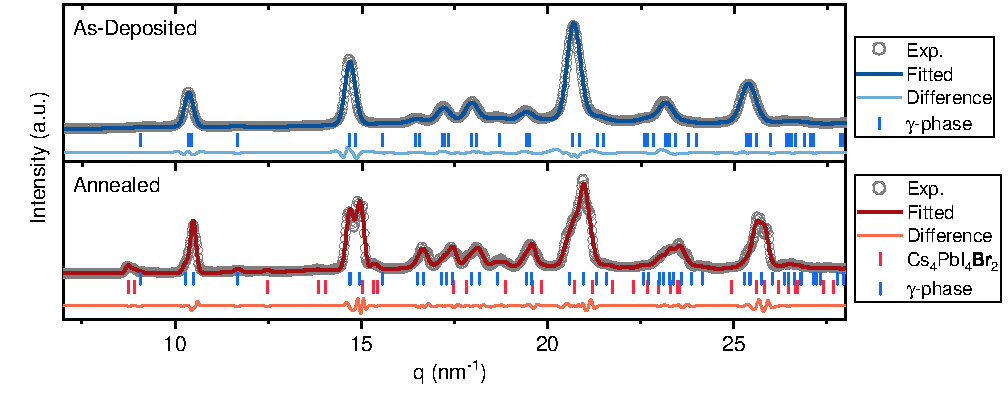
\includegraphics[width=0.85\linewidth]{chapters/material_properties/images/GIWAXS_Before_After.pdf}
        \caption{}
        \label{fig:ch2:giwaxs_before_after:model}
    \end{subfigure}

    \vspace{0.5cm}
    
    % Second image (bottom)
    \begin{subfigure}[b]{\textwidth}
    \centering
    \hspace{-1.4cm}
        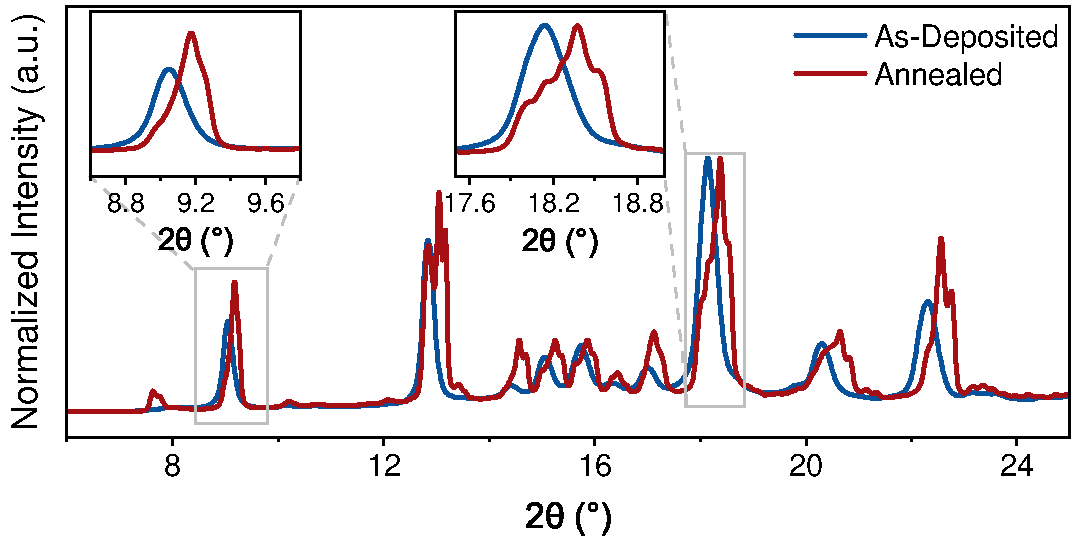
\includegraphics[width=0.68\linewidth]{chapters/material_properties/images/giwaxs_overlayed.pdf}
        \caption{}
        \label{fig:ch2:giwaxs_before_after:overlay}
    \end{subfigure}
    
    \caption[Synchrotron-based GIWAXS of the as-deposited and annealed perovskite state.]{(a) Synchrotron GIWAXS profile and corresponding structural refinement (using a Le Bail fit) for the as-deposited and annealed \ch{CsPbI_2Br} thin film. (b) Overlay comparison of the GIWAXS $2\theta$ signals. The insets highlight three key changes that take place with thermal annealing, including (i) peak shifting, (ii) a reduction of FWHM, and (iii) the appearance of peak splitting. Adapted from \cite{Papadopoulou2024InEllipsometry}.
}
    \label{fig:ch2:giwaxs_before_after:}
\end{figure}



On the other hand, the signal of the annealed perovskite state reveals the co-existence of the $\gamma$-\ch{CsPbI_2Br} phase and a 0D \ch{Cs_4PbX_6} phase, where X indicates the lattice's halogens. The main indicator for the emergence of the 0D phase is the peak that appears at 8.7 $nm^{-1}$. To further investigate the composition of the 0D phase we consider that both \ch{Cs_4PbI_6} and \ch{Cs_4PbBr_6} are stabilized in the same crystal structure (trigonal space group R-3c), which indicates that iodine and bromine can substitute for each other without altering the crystal geometry. Iodine has a larger ionic radius compared to bromine (2.2 {\AA} for $I^-$ compared to 1.96 {\AA} for $Br^-$), meaning that \ch{Cs_4PbI_6} would have larger lattice parameters than \ch{Cs_4PbBr_6} (a = b = 14.602 {\AA}, c = 18.268 {\AA} for the former, and a = b = 13.722 {\AA}, c = 17.299 {\AA} for the latter)\cite{Bhaumik2020BroadbandNanocrystals,DeBastiani2017InsideCrystals}. In our case, the lattice parameters are measured as a = b = 14.138 {\AA}, c = 17.828 {\AA}, clearly indicating that some of the iodine has been replaced by bromine.  Further analysis through Rietveld refinement, including occupancy refinement, confirms a stoichiometry of \ch{Cs_4PbI_4Br_2}. The 0D phase accounted for 10\% of the total perovskite volume, and its formation could potentially be attributed to the the excess of \ch{CsBr} during the co-evaporation process. Nevertheless, the amount of the 0D phase is minimal and unlikely to significantly affect the properties of the main phase \cite{Bai2019AStability}. 

More information about the structure of the annealed and as-deposited state can be extracted through Figure~\ref{fig:ch2:giwaxs_before_after:overlay}, which provides an overlay comparison of the $2\theta$ GIWAXS signals. Through this comparison, three key changes can be observed (i) a reduction in the full width at half maximum (FWHM), (ii) peak shifting, and (iii) the appearance of peak asymmetry or splitting. The FWHM of the peaks is associated with crystallite size, as expressed through Scherrer's equation: 
 \begin{equation}
     D = \frac{k \times \lambda}{\beta \times cos\theta},
 \end{equation}

where k is the shape factor (0.9), $\lambda$ is the X-Ray wavelength, $\beta$ is the FWHM of the peak, and $\theta$ is the the Bragg peak position in radians. This calculation indicates that the crystallite size has nearly doubled as a result of the annealing process, increasing from 16 nm in the as-deposited state to 28 nm for the annealed one. In addition to the increase in crystallite size, the nonuniform peak shift towards the right side and the appearance of peak asymmetry suggest that the annealing process has introduced macrostrain into the system. This strain could be attributed to two main factors: (i) the mismatch in the thermal expansion coefficients between the substrate and the thin film, which can induce biaxial strain at the interface \cite{Steele2019ThermalFilms}, and (ii) the coexistence of the 0D \ch{CsPbI_4Br_2} and the 3D \ch{CsPbI_2Br} phase, which may create lattice anchoring within the system \cite{Steele2022AnFilms, Saha2024Oxygen-MediatedPerformance}

\begin{figure}[htbp]
    \centering
    % First row
    \begin{subfigure}[t]{0.4\textwidth}
        \centering
        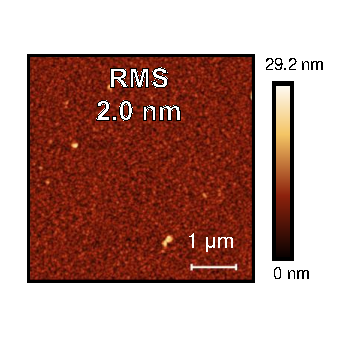
\includegraphics[width=\textwidth]{chapters/material_properties/images/AFM_before.pdf} 
        \caption{}
        \label{fig:ch2:afm_before}
    \end{subfigure}
    \hspace{0.5cm}
    \begin{subfigure}[t]{0.4\textwidth}
        \centering
        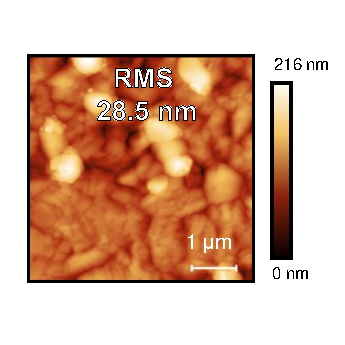
\includegraphics[width=\textwidth]{chapters/material_properties/images/AFM_after.pdf} % Replace with your image file        
        \caption{}
        \label{fig:ch2:afm_after}
    \end{subfigure}

    % Second row
    \begin{subfigure}[t]{0.35\textwidth}
        \centering
        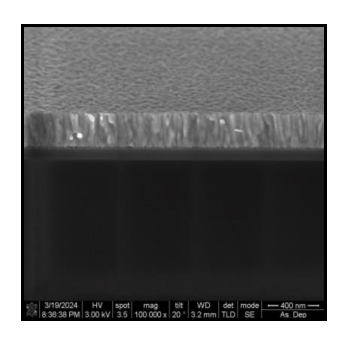
\includegraphics[width=\textwidth]{chapters/material_properties/images/SEM_Before.pdf} 
        \caption{}
        \label{fig:ch2:sem_before}
    \end{subfigure}
    \hspace{1.2cm}
    \begin{subfigure}[t]{0.35\textwidth}
        \centering
        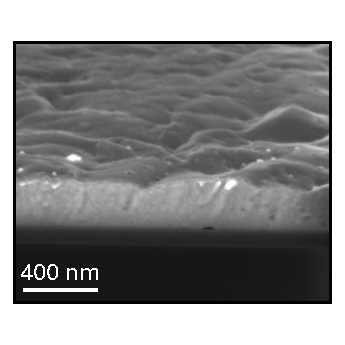
\includegraphics[width=\textwidth]{chapters/material_properties/images/SEM_After.pdf} 
        \caption{}
        \label{fig:ch2:sem_after}
    \end{subfigure}
    \caption[AFM and SEM scans of the as-deposited and annealed perovskite state.]{AFM scans for the (a) as-deposited and (b) annealed perovskite state. SEM cross-section for the (c) as-deposited and (d) annealed perovskite state. Adapted from \cite{Papadopoulou2024InEllipsometry}.}
    \label{fig:ch2:afm_sem}
\end{figure}


Figure~\ref{fig:ch2:afm_sem} demonstrates the impact of this annealing step on the morphology of the perovskite film by comparing the surface morphology and the film's cross-section in the as-deposited and annealed state. The as-deposited state has grains of particularly small size, in the range of 30 - 40 nm (Figure~\ref{fig:ch2:afm_before}), which is in agreement with previous reports on co-evaporated \ch{CsPbI_xBr_{3-x}} thin films \cite{Frolova2017HighlyPbI2, Zhang2023SemitransparentAbsorber}. The RMS roughness is accordingly low and equal to 2 nm. Despite the small grain size, the cross-section of the film (Figure~\ref{fig:ch2:sem_before}), shows a compact morphology without any noticeable defects, cracks or pinholes. The annealing step has a major effect on the morphology of the film, yielding a broad distribution of grain sizes, between 100 and 800 nm in diameter, as shown in the respective AFM image (Figure~\ref{fig:ch2:afm_after}). The surface roughness has increased to 28.5 nm. At the same time, the SEM scan (Figure~\ref{fig:ch2:sem_after}) reveals a grain-boundary-free cross-section, which is typically associated with improved optoelectronic properties. 




\begin{figure}[ht!]
    \centering
    % First row
    \begin{subfigure}[t]{0.4\textwidth}
        \centering
        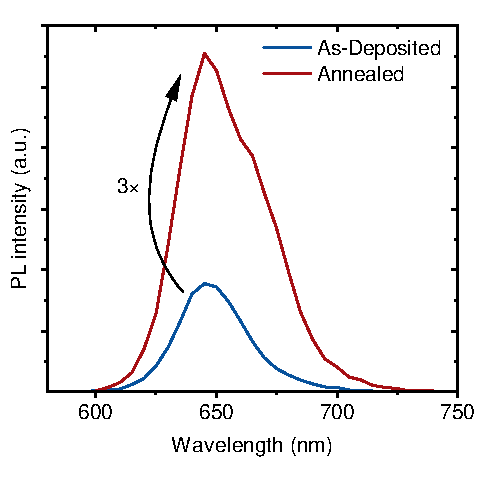
\includegraphics[width=\textwidth]{chapters/material_properties/images/SSPL.pdf} 
        \caption{}
        \label{fig:ch2:sspl}
    \end{subfigure}
    \hspace{1cm}
    \begin{subfigure}[t]{0.4\textwidth}
        \centering
        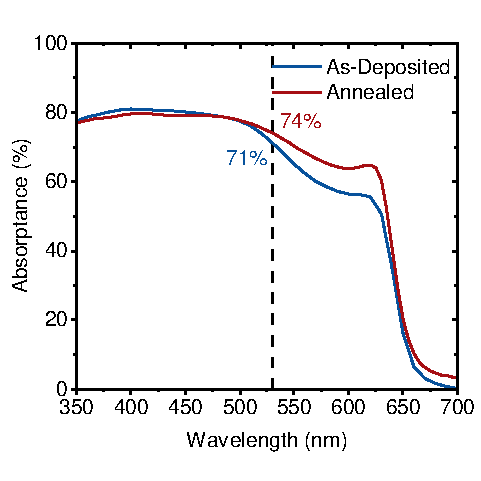
\includegraphics[width=\textwidth]{chapters/material_properties/images/Absorptance.pdf} % Replace with your image file
        \caption{}
        \label{fig:ch2:absorptance}
    \end{subfigure}

    \vspace{1em} % Space between rows

    % Second row
    \begin{subfigure}[t]{0.4\textwidth}
        \centering
        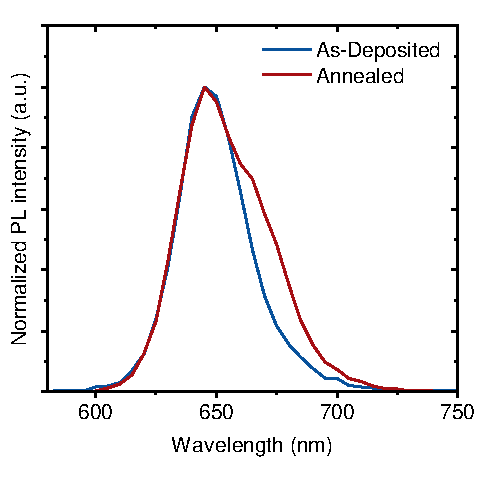
\includegraphics[width=\textwidth]{chapters/material_properties/images/SSPL_norm.pdf} % Replace with your image file
        \caption{}
        \label{fig:ch2:norm_sspl}
    \end{subfigure}
    \hspace{1cm}
    \begin{subfigure}[t]{0.4\textwidth}
        \centering
        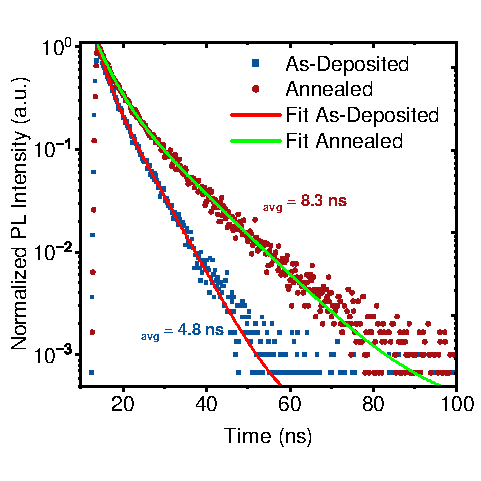
\includegraphics[width=\textwidth]{chapters/material_properties/images/TRPL_norm_double - Copy.pdf} % Replace with your image file
        \caption{}
        \label{fig:ch2:trpl}
    \end{subfigure}
    \caption[SSPL, TRPL, and absorptance of the as-deposited and annealed perovskite state.]{Comparison of the (a) SSPL spectra, (b) absorptance spectra, (c) normalized SSPL spectra, and (d) TRPL signals for the as-deposited and annealed perovskite state. Reproduced from \cite{Papadopoulou2024InEllipsometry}.}
\end{figure}



To further investigate the impact of the annealing step on the optoelectronic properties of the film, we deposit an identical perovskite film on a glass substrate and repeat the same annealing step, which allowed us to perform steady and transient state photoluminescence (SSPL and TRPL), as well as absorptance measurements for the as-deposited and annealed perovskite state. The SSPL measurement in Figure~\ref{fig:ch2:sspl}, indicates a 3-time increase in the intensity of the PL signal for the annealed film under a 530 nm excitation. This could potentially be attributed to increased absorptance at the excitation wavelength or to a reduction of the non-radiative recombination pathways. The absorptance of the annealed film is indeed slightly higher at 530 nm, as demonstrated in Figure~\ref{fig:ch2:absorptance}, however it is not sufficient to justify the increase in PL intensity. Therefore, the increase in crystallite size and the reduction of grain boundaries, as discussed above, contributed to minimizing non-radiative recombination mechanisms. It has to be noted, that there is no indication for the high-bandgap 0D \ch{Cs_4PbI_4Br_2} phase in the SSPL or absorptance spectra of the perovskite. This is in agreement with what was previously reported by Bai et al., who were able to detect the 0D phase in the absorptance spectrum only for highly non-stoichiometric films \cite{Bai2019AStability}. 

When comparing the normalized PL peaks for the as-deposited and annealed perovskite state, in Figure~\ref{fig:ch2:norm_sspl}, an additional difference is observed, with the annealed film exhibiting a secondary, red-shifted shoulder in its PL emission spectrum. This phenomenon was extensively studied by Schötz et al., and was attributed to a self-absorption mechanism, whose impact is amplified by strong internal emissions and the perovskite's Urbach tail \cite{Schotz2020DoubleSelf-absorption}. As a result, the increase in surface roughness that is introduced during the annealing of our thermally evaporated perovskite could explain the double peak emission via an increase in internal light scattering. Lastly, Figure~\ref{fig:ch2:trpl} shows the TRPL spectra for the as-deposited and annealed perovskite state. A bi-exponential equation, described by the formula: 

\begin{equation}
    I_{PL}(t) = A_1exp(-\frac{t}{\tau_1}) + A_2exp(-\frac{t}{\tau_2}) + y_0,
\end{equation}

was able to accurately describe the decay of the both curves. Followingly, the average lifetime of the carriers was calculated using the equation: 
\begin{equation}
    \tau_{avg} = \frac{A_1 \tau_1^2 + A_2 \tau_2^2}{A_1 \tau_1 + A_2 \tau_2},
\end{equation}

indicating an almost doubling of the carriers' lifetime, from 4.8 ns for the as-deposited state to 8.3 ns for the annealed one.

\begin{figure}
  \centering
  \medskip
  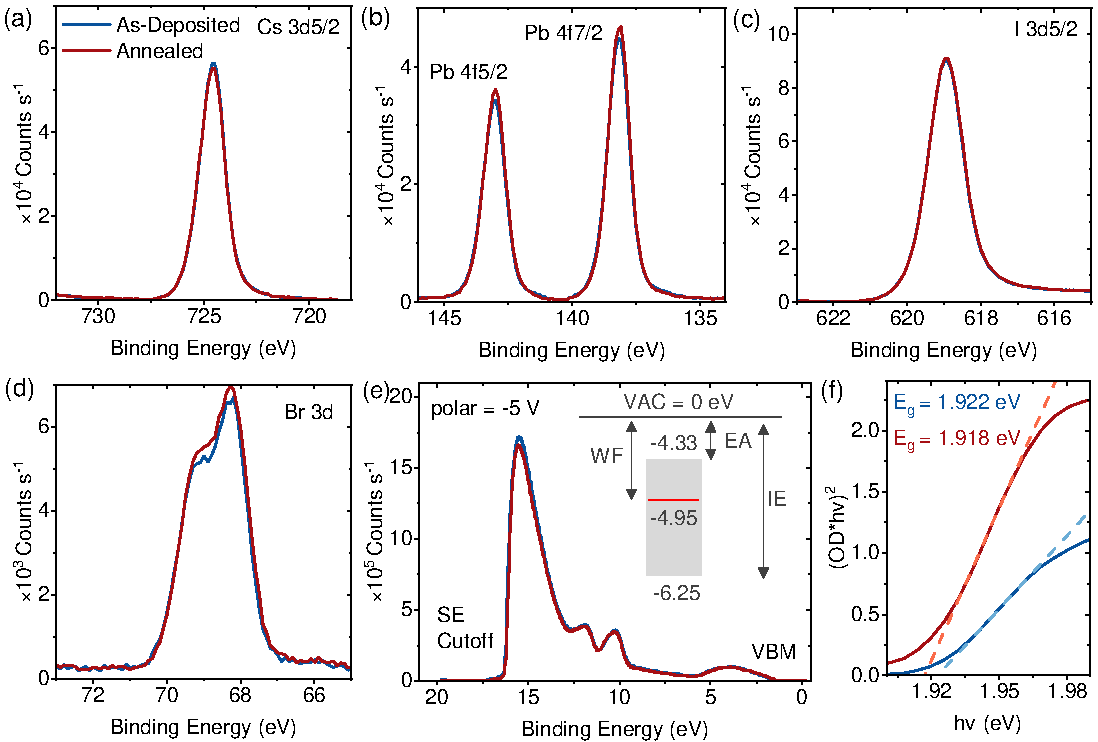
\includegraphics[width=0.9\textwidth]{chapters/ellipsometry/image/UPS_XPS_Eg.pdf}
  \caption[XPS and UPS signals of the as-deposited and annealed perovskite state.]{XPS narrowband spectra of (a) Cs3d5/2, (b) Pb4f5/2 and Pb4f7/2, (c) I3d5/2, and (d) Br3d for the as-deposited (blue) and annealed (red) perovskite state. (e) Full UPS spectra of the as-deposited and annealed perovskite state. The index illustrates the energy band diagram of the samples. (f) Tauc plot derived from UV-Vis absorption measurements, used to determine the optical bandgap of the as-deposited and annealed perovskite films. OD represents the films’ optical density.} 
  
  \label{fig:ch3:ups_xps}
\end{figure}

Lastly, the chemical composition of the as-deposited and annealed perovskite films was investigated using X-ray photoelectron spectroscopy (XPS) (Figure~\ref{fig:ch3:ups_xps}a–d). The absence of binding energy shifts and the preservation of peak shapes indicate that no significant chemical changes occur during the thermal annealing process. Quantitative analysis based on peak area integration yields a composition of \ch{Cs_{1.25}PbI_{1.82}Br_{0.97}}, suggesting a Cs:Pb ratio higher than the nominal value (1.05:1.00). It is important to note that XPS probes only the surface of the perovskite layer, and this stoichiometry may differ from that of the bulk. It is also worth considering that additional changes in the sample's surface stoichiometry may be induced by the surface cleaning step, via a sequential gas cluster ion beam sputtering, before the XPS measurement. Furthermore, ultraviolet photoelectron spectroscopy (UPS) measurements (Figure~\ref{fig:ch3:ups_xps}e) show that the electronic structure remains unchanged upon annealing. The work function (WF) and ionization energy (IE) were determined to be -4.95 eV and -6.25 eV, respectively. With an optical bandgap of approximately 1.92 eV for both films (Figure~\ref{fig:ch3:ups_xps}f), the resulting electron affinity (EA) is calculated to be -4.33 eV.

\section{In-Situ Investigation via Spectroscopic Ellipsometry} \label{sec:in_situ}

Besides the comparison of the properties between the as-deposited and annealed state at RT, valuable information about the film can be extracted through in-situ measurements. A characteristic example is in-situ GIWAXS, which due to its fast acquisition time, allows for the monitoring of crystal changes in real time with increasing temperature. Such results for our co-evaporated \ch{CsPbI_2Br} thin films are presented in Figure~\ref{fig:ch2:giwaxs_insitu}, which shows the in situ reduced 1D GIWAXS data during the temperature heating ramp. The transition from the orthorhombic ($\gamma$-) to the tetragonal ($\beta$-) phase is found to take place close to 130 \degree C, while the transition to the cubic ($a$-) phase happens at approximately 190 \degree C. Lastly, the emergence of the peak at 8.7 $nm^{-1}$ at 225 \degree C indicates the emergence of the 0D \ch{Cs_4PbI_4Br_2} phase. 


While knowledge of phase transition temperatures is crucial for optimizing the post-deposition annealing step, relying on synchrotron-based techniques such as GIWAXS presents challenges due to their high costs and limited accessibility. Therefore, developing an alternative, in-house characterization technique capable of providing real-time insights into the annealing effects on perovskite thin films would be highly beneficial. This technique must be compatible with the soft nature of perovskite films, operable in a controlled environment, and capable of functioning at various temperatures. Additionally, it must have a sufficiently fast acquisition rate to detect real-time changes.

All of these conditions are met by spectroscopic ellipsometry, a fast, non-destructive characterization technique that provides a wealth of information on both the structural and optical properties of thin films, and is accessible to the vast majority of nanotechnology facilities. When combined with a heating stage and gas flow for a controlled environment, it can simulate various annealing conditions of perovskite thin films. The following sections lay the foundational principles of spectroscopic ellipsometry before elaborating on the challenges of temperature-dependent measurements. A novel dynamic modeling approach is proposed, which is then used to investigate the real-time temperature effect on the structural and optical properties of \ch{CsPbI_2Br} thin films. Through this analysis, it is possible not only to quantify critical parameters such as the film's thickness, roughness, and optical constants as a function of temperature, but also to identify indicators that reveal phase changes. Furthermore, through additional data manipulation, we quantitatively assess the film's Urbach energy and thermo-optic coefficient.


\begin{figure}
  \centering
  \medskip
  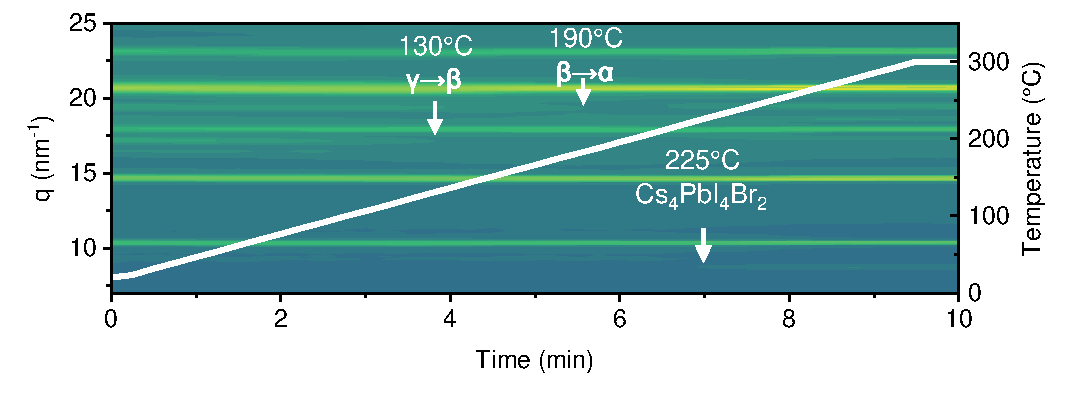
\includegraphics[width=\textwidth]{chapters/material_properties/images/GIWAXS_In_Situ.pdf}
  \caption[In situ reduced 1D GIWAXS data of the \ch{CsPbI_2Br} film during the thermal annealing heating ramp.]{In situ reduced 1D GIWAXS data during the thermal annealing heating ramp. Arrows indicate the phase transitions, as well as the emergence of the 0D \ch{Cs_4PbI_4Br_2} phase. Reproduced from \cite{Papadopoulou2024InEllipsometry}.} 
  
  \label{fig:ch2:giwaxs_insitu}
\end{figure}



\subsection{Fundamentals of Spectroscopic Ellipsometry} \label{ch:ellipsometry:intro}


Spectroscopic ellipsometry (SE) is a widely used optical characterization technique, suitable for the determination of a thin film's thickness, roughness, optical constants, and more. Its working principle can be summarized as follows: 

\begin{enumerate}[i.]
  \item A linearly polarized light source is directed at a thin-film-coated substrate.
  \item The reflection and transmission of the incident light at the sample are governed by the Fresnel equations.
  \item The reflected light becomes elliptically polarized, meaning that the oscillatory directions of the electric field parallel (\textit{p}-plane) and perpendicular (\textit{s}-plane) to the incident plane are out of phase and have different amplitude.
  \item The reflected light gets detected by a polarization detection system.
\end{enumerate}

This change in polarization is described by two parameters, namely $\Psi$ and $\Delta$, which represent the amplitude ratio and phase difference between the p- and s-polarizations, respectively. This is summarized in equation: 

\begin{equation}
\frac{r_p}{r_s} = \tan(\Psi) \cdot e^{i\Delta},
\label{eq:ellipsometry}
\end{equation}

where $r_p$ and $r_s$ describe the reflection coefficient for the \textit{p}-polarized and \textit{s}-polarized light, respectively \cite{Fujiwara2018SpectroscopicCharacterization}.

\begin{figure}{}
  \centering
  \medskip
  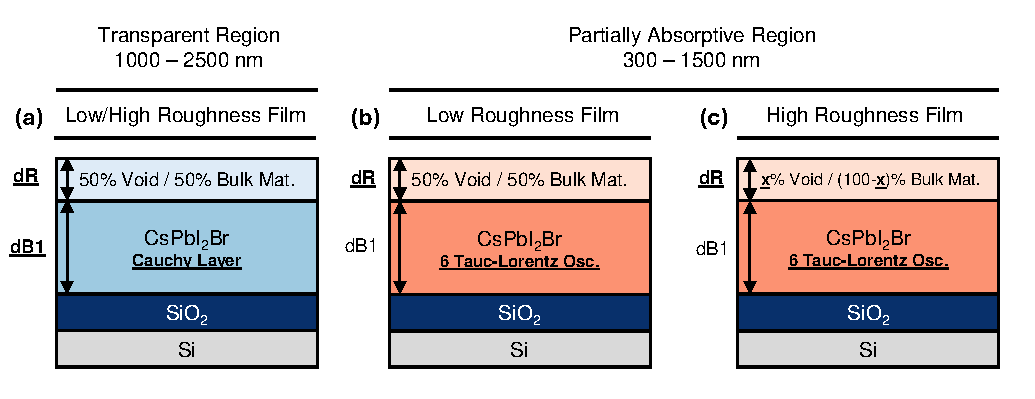
\includegraphics[width=.95\textwidth]{chapters/ellipsometry/image/Model_Approach.pdf}
  \caption[Schematic illustration of the modeling approach for SE data, depending on the roughness of the studied film.]{Schematic illustration of the modeling approach for SE data, depending on the roughness of the studied film. Bold and underlined text indicates the fitting parameters of each optical model. (a) The bulk perovskite thickness (dB1) for both low and high roughness films is extracted through a Cauchy model in the film's transparent region. The optical constants are followingly extracted through a Tauc-Lorentz Gen. Osc. model in the partially absorptive region with the percentage of voids in the roughness layer set (b) to 50\% for low roughness films and (c) as a fitting parameter for high roughness films. Reproduced from \cite{Papadopoulou2024InEllipsometry}.}
  \label{fig:ellipsometry:static_models}
\end{figure}

SE data are typically collected across a wide range of wavelengths (300 nm - 2500 nm) and at various angles of incidence (between 45\degree and 85\degree). This relatively simple dataset contains ample information about the physical material properties of a thin film (including its thickness, roughness, dielectric functions, uniformity, composition, and more), however a careful model-based regression analysis is required to extrapolate them. This means that a model of the sample has to be created, which consists of fixed and fitted parameters. Fixed parameters are the known samples properties (e.g. the dielectric function of the substrate), while fitted parameters are all the unknown properties that are under investigation. An initial "guessing" of these unknown properties is necessary, followed by an iterative data-fitting process that compares the simulated and experimental $\Psi$ and $\Delta$ values. In the end, the quality of the fitting process is described by the mean squared error (MSE), given by: 


\begin{equation}
MSE = \sqrt{ \frac{1}{3n - m} \sum_{i=1}^{n} \left[ 
\left( \frac{N_{E_i} - N_{G_i}}{0.001} \right)^2 + 
\left( \frac{C_{E_i} - C_{G_i}}{0.001} \right)^2 + 
\left( \frac{S_{E_i} - S_{G_i}}{0.001} \right)^2 
\right] }
\label{eq:mse}
\end{equation}

where  "n" is the number of wavelengths, "m" is the number of fit parameters, and N=cos(2$\Psi$), C=sin($2\Psi$)cos($\Delta$), S=sin($2\Psi$)sin($\Delta$). Measured data are denoted with the subscript "E", while model generated data are denoted with subscript "G". Typically, achieving an MSE that is as low as possible is the objective. In the framework of this study, an MSE below 20 is considered necessary to ensure a good match between experimental and simulated values. 


For the characterization of perovskite thin films via spectroscopic ellipsometry, the following protocol can be followed for a foolproof model development: 
\begin{itemize}
    \item The spectral range is limited to a region where the perovskite film is transparent, i.e. below its bandgap value. In the case of our thermally evaporated \ch{CsPbI2Br} thin films (\ch{E_g} = 645 nm), we limit the spectral range between 1000 and 2500 nm. 
    \item In this region, the extinction coefficient (k) of the material is equal to 0, so the response of the material can be solely described by its refractive index (n), via the empirical Cauchy dispersion model:
        \begin{equation}
            n(\lambda) = A + \frac{B}{\lambda^2} + \frac{C}{\lambda^4}
            \label{eq:cauchy}
        \end{equation}
    \item Besides the A, B, and C values of equation \ref{eq:cauchy}, additional fitting parameters include the thickness of the perovskite bulk and the thickness of the roughness layer (as shown in Figure~\ref{fig:ellipsometry:static_models}a). The roughness is typically simulated as an additional layer, which follows the Bruggeman effective medium approximation (EMA), consisting of 50\% voids and 50\% bulk material, as introduced by Aspens et al \cite{Aspnes1979InvestigationEllipsometry}. 

    \item The Cauchy model is ideal for a good estimation of the bulk's thickness owing to (i) relatively low number of fitting parameters, (ii) the interference of light reflected both from the sample's surface and the interface with the substrate, and (iii) the small influence of surface roughness in the infrared region.

    \item Having now bulk thickness as a fixed parameter, the Cauchy layer can be parameterized into a Kramers-Kroning consistent B-spline layer, extending the SE data range to the visible spectrum (up to 300 nm). 

    \item As a last step, the bulk's dielectric constant is further parameterized into a General Oscillator layer. (Figure~\ref{fig:ellipsometry:static_models}b).    

\end{itemize}

Choosing the right type and number of oscillators in the last step is critical for the accurate determination of the film's optical constants. Using too few oscillators might make it impossible to reproduce the features in the experimental data, while using too many oscillators might lead to overfitting and the generation of results with little physical meaning. For the modeling of semiconductor materials, the use of Gaussian oscillator is the simplest choice. The imaginary part of the dielectric constant ($\varepsilon_r$) can be described by three free parameters, namely the amplitude ($A$), the broadening ($C$), and the center energy ($E_0$). However, the symmetric nature of the Gaussian oscillator does not fully describe the real optical transitions is thin films, where tail states and disorder lead to asymmetric broadening. As an alternative, Tauc-Lorentz oscillators are more commonly used for the modeling of perovskite thin films. This type of oscillator has one additional parameter that describes the bandgap energy of the material ($E_g$), producing a more asymmetric and realistic $\varepsilon_2$ shape \cite{Jellison1996ParameterizationRegion}. Therefore, the absorption from the Tauc-Lorentz oscillator is described by: 

\begin{equation}
\varepsilon_2(E) =
\begin{cases}
\frac{A E_0 C}{E} \cdot \frac{(E - E_g)^2}{(E^2 - E_0^2)^2 + C^2 E^2}, & E > E_g \\
0, & E \leq E_g
\end{cases}
\label{eq:tauc_lorentz}
\end{equation}

\begin{figure}[tbp]
  \centering
  \medskip
  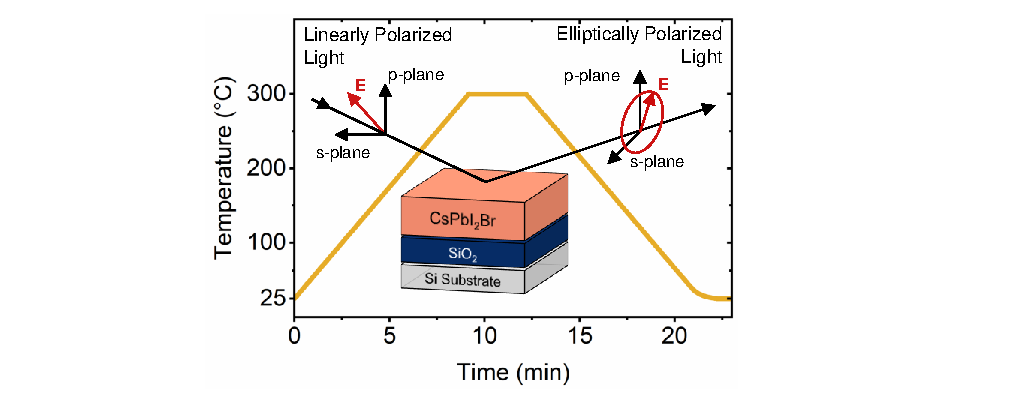
\includegraphics[width=.99\textwidth]{chapters/ellipsometry/image/experiment_description.pdf}
  \caption[Schematic illustration of the temperature-dependent in situ SE characterization measurement.]{Schematic illustration of the temperature-dependent in situ SE characterization measurement. Reproduced from \cite{Papadopoulou2024InEllipsometry}.}
  \label{fig:ellipsometry:experiment_description}
\end{figure}


The properties of perovskite thin films have been widely studied by means of SE measurements in literature. When measurements were performed in room temperature (RT), they were mainly used for the determination of the complex optical constants for various perovskite compositions \cite{Yan2020DeterminationFilms, Zhao2018EllipsometricFilm, Loper2015ComplexSpectrophotometry, Yuan2021Moisture-stimulatedProperties}. In a few occasions, SE in room temperature was used for less common studies, such as the identification of light-induced phase segregation \cite{Bernhardt2022InPerovskites} or the evaluation of perovskite degradation under ambient conditions \cite{Marronnier2018ElectricalConditions}. On the other hand, temperature-dependent SE measurements were previously performed on perovskite thin films for the characterization of their temperature-dependent optical properties \cite{Jiang2016TemperatureEllipsometry, Chen2019CharacterizingEllipsometry}, the investigation of temperature-induced degradation \cite{Tejada2022HybridInfrared, Wang2019InEllipsometry}, and the identification of phase-transition temperatures \cite{Yuan2020InPortfolio, Yuan2021Moisture-stimulatedProperties}. The following sections will identify specific limitations in the modeling of temperature-dependent SE data, present a novel dynamic modeling approach, and lastly provide new insights into the in situ annealing effect on thermally evaporated \ch{CsPbI2Br} thin films.  


\subsection{Temperature-Dependent Spectroscopic Ellipsometry}



\begin{figure}[ht!]
    \centering
    % First plot
    \begin{subfigure}[t]{0.9\textwidth} % Adjust width if needed
        \centering
        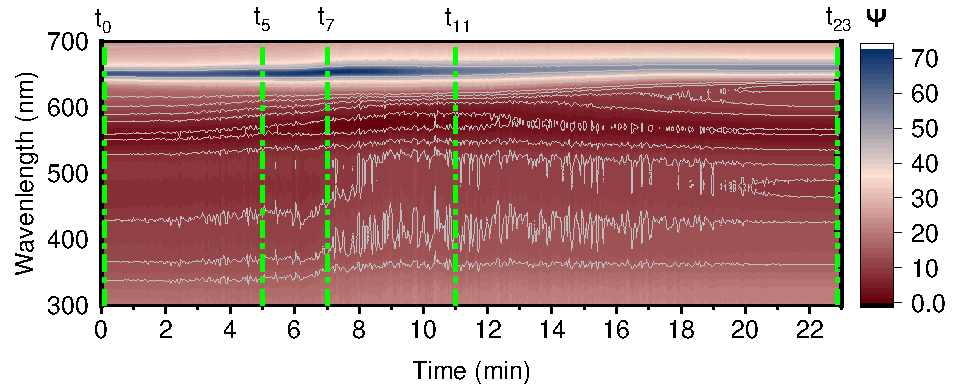
\includegraphics[width=\textwidth]{chapters/ellipsometry/image/Psi_Contour - MRS.pdf} % Replace with your image
        %\caption{Description for subplot (a).}
        %\label{fig:sub-a}
    \end{subfigure}

    \vspace{1em} % Space between the rows

    % Second plot
    \begin{subfigure}[t]{0.9\textwidth} % Adjust width if needed
        \centering
        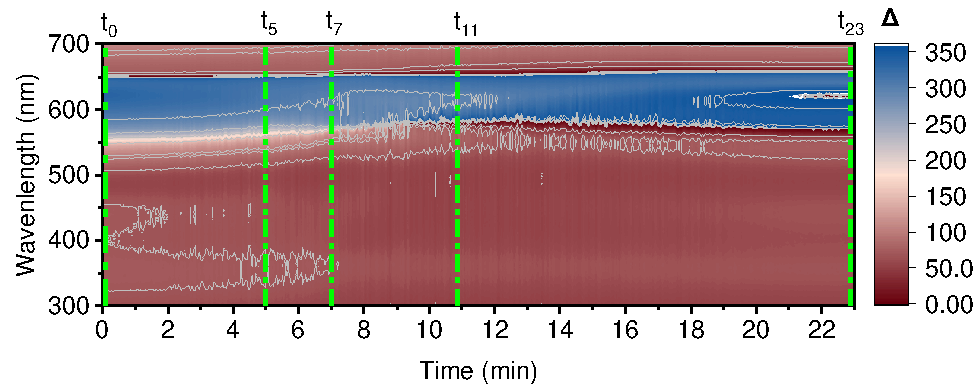
\includegraphics[width=\textwidth]{chapters/ellipsometry/image/Delta_Contour - MRS.pdf} % Replace with your image
        %\caption{Description for subplot (b).}
        %\label{fig:sub-b}
    \end{subfigure}

    % Caption for the whole figure
    \caption[Evolution of $\Psi$ and $\Delta$ as a function of time and temperature]{Evolution of $\Psi$ and $\Delta$ as a function of time (and temperature). The wavelength range has been limited to 300 - 700 nm for a more clear visualization. The green dashed lines mark the timestamps for which a static model was developed. Reproduced from \cite{Papadopoulou2024InEllipsometry}.}
    \label{fig:ellipsometry:raw_psi_delta}
\end{figure}

Most studies on temperature-dependent SE characterization follow an approach where they change the sample's temperature in step-wise increments or decrements, allowing for some stabilization time before moving to the next temperature step. A separate SE model is then developed for each temperature step. While this methodology ensures adequate time for potential transitions or internal structure changes, it is also likely that to conceal information around real-time effects. As an alternative, the implementation of a continuous heating ramp could be more representative of the changes that are taking place during a real annealing step. For this reason, we implemented the heating ramp shown in Figure~\ref{fig:ellipsometry:experiment_description} for the characterization of an  \ch{CsPbI2Br} thin film, deposited on a Si substrate with 100 nm of thermally grown \ch{SiO_2}. This choice of substrate prevents complications arising from backside reflection in semitransparent substrates or multilayer interference within multilayer stacks. The sample was placed in a enclosed temperature stage that was continuously flushed with nitrogen. Starting from RT, the temperature was increased with a rate of approximately 30\degree C/min, up to 300\degree C. The sample was allowed to stabilize there for 3 minutes, before being cooled back down to RT with a rate of 35\degree C/min. An SE measurement at a fixed incident angle of 70\degree was taken approximately every 1.3 seconds. It would not be possible to perform varied angle SE due to the fixed position of the optical windows on the heating stage. The acquired $\Psi$ and $\Delta$ values
as function of time are shown in Figure~\ref{fig:ellipsometry:raw_psi_delta}. Even though this data give some high level information about the moments the sample is going through drastic changes (e.g. between the $5^{\text{th}}$ and $11^{\text{th}}$ minute of the experiment), a careful modeling is necessary to decipher them. 

\begin{figure}
  \centering
  \medskip
  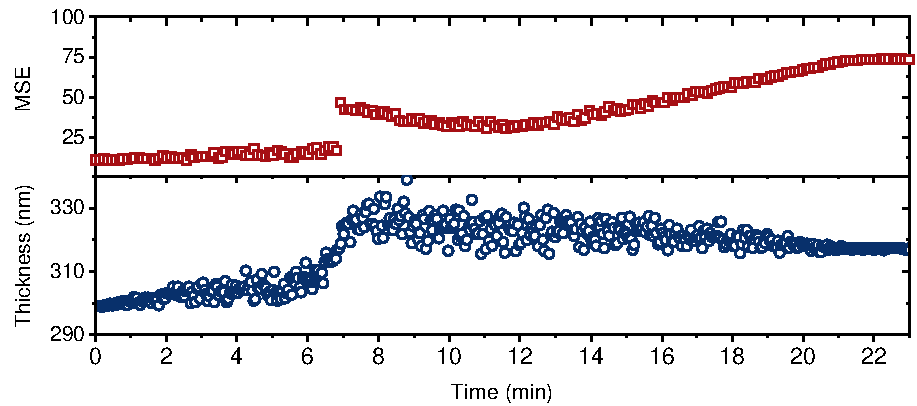
\includegraphics[width=.77\textwidth]{chapters/ellipsometry/image/wrong_model.pdf}
  \caption[Example of inaccurate modeling of dynamic SE data resulting from the use of a single optical model with all parameters fitted as a function of time.]{Example of inaccurate modeling of dynamic SE data resulting from the use of a single optical model with all parameters fitted as a function of time.}
  \label{fig:ellipsometry:wrong_model}
\end{figure}

However, the modeling of continuous SE data is not straightforward. One option that is facilitated by the software used for the analysis of the SE data (CompleteEASE) is the development of a static model for the initial state of the sample ($t_0$) (according to the protocol described in the previous section), followed by the dynamic fitting of its parameters as a function of time. We can expect that the thickness of the sample is changing due to thermal expansion, its roughness is increasing due to grain coalescence, and the position/energy of the oscillators are changing due to the energy that is transferred to the system. Therefore, for such a modeling approach 26 fitting parameters (1$\times$thickness, 1$\times$roughness, 6$\times$4 oscillators) should be turned-on. The continuous fitting of such a system is not only computationally heavy, but also entails the risk of overfitting. Some indicative results of such a modeling approach are demonstrated in Figure~\ref{fig:ellipsometry:wrong_model}. Despite the fact that at the start of the experiment the MSE is reasonably low at the beginning of the measurement, it rises above 70 by the end of the experiment, pointing out to a large difference between measured and simulated data. Additionally, the predicted thickness of the film in the end of the measurement is almost 20 nm higher compared to the thickness of the as-deposited film. This is in contradiction with the profilometry results for the as-deposited and annealed state of the sample, which have approximately the same thickness, as shown in Figure~\ref{fig:ellipsometry:profilometry}. Therefore, the continuous fitting of the initial static model is an unreliable way to model the acquired results. 


\begin{figure}
  \centering
  \medskip
  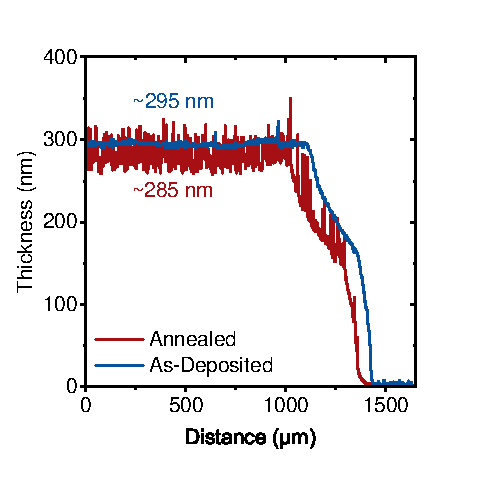
\includegraphics[width=.45\textwidth]{chapters/ellipsometry/image/Dektak.pdf}
  \caption[Thickness comparison for the as-deposited and annealed perovskite film, measured via profilometry.]{Thickness comparison for the as-deposited and annealed perovskite film, measured via profilometry. The film thickness is approximated based on the step height as the profilometer stylus traverses from the perovskite film to the uncoated substrate. Reproduced from \cite{Papadopoulou2024InEllipsometry}.}
  \label{fig:ellipsometry:profilometry}
\end{figure}

An alternative modeling approach was inspired by a previous report on the modeling of aluminum gallium arsenide (\ch{Al_xGa_1_-_xAs}) optical constants as a function of composition \cite{Snyder1990ModelingComposition}. Specifically, considering that, for example, the optical constants of the compositions for $x=0.3$ and $x=0.4$ are known, then the optical constants of the intermediate composition for $x=0.35$ could be simulated as a mixture (via the effective medium approximation model - EMA) of the two known compositions. Extending this concept to our experiment, we identified that it is possible to describe the complete temperature-dependent evolution of the perovskite thin film via a mixture of its optical constants at selected timestamps. This can be described by an EMA-based model, as shown in Figure~\ref{fig:ellipsometry:dynamic_model}, where the bulk of the perovskite layer is a mixture of five static models, namely $sm1-t_0$, $sm-t_5$, $sm-t_7$, $sm-t_{\text{11}}$, and $sm-t_{\text{23}}$. The names of these static models represent the time frame they refer to, and they can be further distinguished in Figure~\ref{fig:ellipsometry:raw_psi_delta}. The oscillator parameters of each static model are fixed. Only the volume fraction of each static model along with the bulk thickness and roughness thickness are set as fitting parameters. This creates a lightweight dynamic model with only 7 fitting parameters in total that can be fit in real time. The selection of these specific five static models was intentional: $sm1-t_0$ and $sm-t_{\text{23}}$ were included to account for the as-deposited and annealed state at RT, while $sm-t_{\text{11}}$ was included to account for the perovskite state at 300\degree C. Lastly, $\Psi$ and $\Delta$ values reveal that a major shift is happening to the composition of the perovskite around the $6^{\text{th}}$ minute of the experiment, motivating us to include two additional static models ($sm-t_5$ and $sm-t_7$) to account for the perovskite state before and after this shift. An essential condition for the accuracy of the dynamic EMA model is the accuracy of the constituents static models. For this reason, the following section provides a comprehensive analysis on the development of the static models, particularly for the as-deposited ($sm1-t_0$) and the annealed ($sm-t_{\text{23}}$) perovskite state, highlighting the impact of the surface roughness on the accuracy of simulated results. We specifically focus on the as-deposited and annealed state since the simulated results can be further corroborated through additional characterizations measurements before and after the annealing of the perovskite thin film. 

\begin{figure}
  \centering
  \medskip
  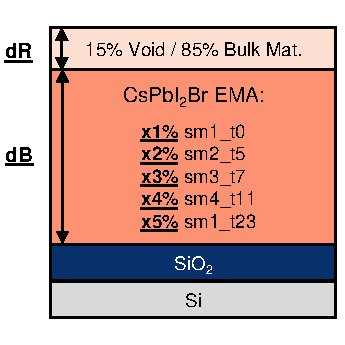
\includegraphics[width=.4\textwidth]{chapters/ellipsometry/image/Dynamic_Model.pdf}
  \caption[Schematic of the optical model used for the fitting of dynamic SE data.]{Schematic of the optical model used for the fitting of dynamic SE data. The bulk layer consists of five static models, which have been developed for the timestamps shown in Figure~\ref{fig:ellipsometry:raw_psi_delta}. Only the volume fraction of these static models is set as a fitting parameter. Additional fitting parameters are the thickness of the bulk and the roughness layers. The percentage of voids in the roughness layer is set to 15\%. Reproduced from \cite{Papadopoulou2024InEllipsometry}.}
  \label{fig:ellipsometry:dynamic_model}
\end{figure}



\subsection{Static and Dynamic Model Development}

\begin{figure}[t]
    \centering
    % First row
    \begin{subfigure}[t]{0.4\textwidth}
        \centering
        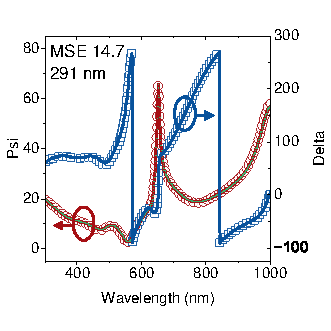
\includegraphics[width=\textwidth]{chapters/ellipsometry/image/t0_plot.pdf} % Replace with your image file
        \caption{}
        \label{fig:ellipsometry:static_fits:t0}
    \end{subfigure}
    \hspace{1cm}
    \begin{subfigure}[t]{0.4\textwidth}
        \centering
        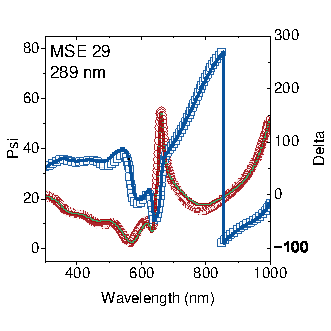
\includegraphics[width=\textwidth]{chapters/ellipsometry/image/t23_fixed_thickness_50_v.pdf} 
        % Replace with your image file
        \caption{}
        \label{fig:ellipsometry:static_fits:t23_fixed_thick_50_void}
    \end{subfigure} 
 % Second row
    \begin{subfigure}[t]{0.4\textwidth}
        \centering
        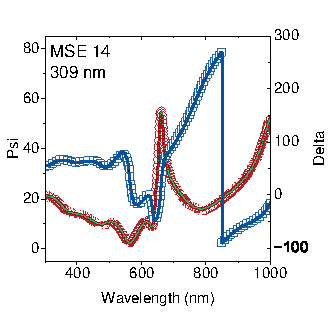
\includegraphics[width=\textwidth]{chapters/ellipsometry/image/t23_fitted_thickness.pdf} % Replace with your image file
        \caption{}
        \label{fig:ellipsometry:static_fits:t23_fitted_thick}
    \end{subfigure}
    \hspace{1cm}
    \begin{subfigure}[t]{0.4\textwidth}
        \centering
        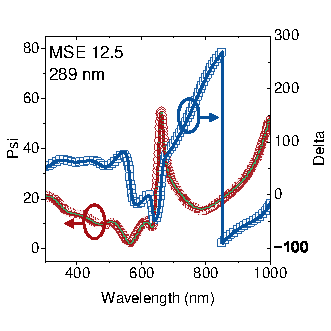
\includegraphics[width=\textwidth]{chapters/ellipsometry/image/t23_fixed_thick_x_void_p.pdf} % Replace with your image file
        \caption{}
        \label{fig:ellipsometry:static_fits:t23_fixed_thick_x_void}
    \end{subfigure}
    \caption[Comparison between the experimental (scatter points) and simulated (solid lines) SE results for the as-deposited and annealed perovskite states.]{Comparison between the experimental (scatter points) and simulated (solid lines) SE results for the as-deposited and annealed perovskite states. The MSE and the simulated bulk thickness are also indicated for (a) the as-deposited film (fixed bulk thickness and 50\% voids in the roughness layer) and annealed film, simulated with (b) fixed bulk thickness and 50\% voids in the roughness layer (c) fitted bulk thickness and 50\% voids in the roughness layer, and (d) fixed bulk thickness and fitted \% of voids in the roughness layer. Adapted from \cite{Papadopoulou2024InEllipsometry}.}
    \label{fig:ellipsometry:static_fits}
\end{figure}

Developing a model for the as-deposited state ($sm1-t_0$) is rather straight forward, due to the relatively low surface roughness of the film (RMS = 2~nm, as seen in Figure~\ref{fig:ch2:afm_before}). We consider that the interface between \ch{SiO_2} and \ch{CsPbI_2Br} is smooth with no intermixing between the layers. Following the protocol described in Section \ref{ch:ellipsometry:intro}, we extract a bulk thickness via a Cauchy model in the transparent region and get an approximation of 291 nm, which is consistent with the value provided by profilometry (295 nm in Figure~\ref{fig:ellipsometry:profilometry}). The dielectric function of the film in the absorptive region is then modeled using 6 Tauc-Lorentz Oscillators, as shown in Figure~\ref{fig:ellipsometry:static_models}, while the surface roughness is simulated through an additional EMA layer that consists of 50\% voids and 50\% bulk material. The fitting results of the $\Psi$ and $\Delta$ values are shown in Figure~\ref{fig:ellipsometry:static_fits:t0}, where a good agreement between measurement and simulation is indicated via a relatively low MSE, equal to 14.7. To further corroborate the accuracy of the simulation, we extract the nk values for the as-deposited state and use them to simulate the film's absorptance and reflectance using the transfer matrix algorithm. Next, we experimentally evaluate the same parameters, via Reflectance/Transmittance measurements (R/T), considering the formula A(\%) = 100 - R(\%) - T(\%), where A stands for the film's absorptance. Figure~\ref{fig:ellispometry:rt_as_dep} demonstrates a good agreement between experimental and simulated values, further corroborating the accuracy of the static model $sm1-t_0$.


\begin{figure}[htbp]
    \centering
    % First plot
    \begin{subfigure}[t]{0.4\textwidth} % Adjust width as needed
        \centering
        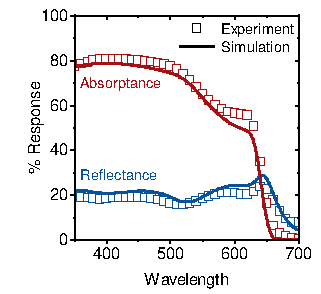
\includegraphics[width=\textwidth]{chapters/ellipsometry/image/RT_As_Deposited.pdf} % Replace with your image
        \caption{}
        \label{fig:ellispometry:rt_as_dep}
    \end{subfigure}
    \hspace{1cm}
    % Second plot
    \begin{subfigure}[t]{0.4\textwidth} % Adjust width as needed
        \centering
        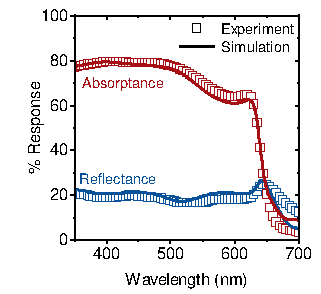
\includegraphics[width=\textwidth]{chapters/ellipsometry/image/RT_Annealed.pdf} % Replace with your image
        \caption{}
        \label{fig:ellipsometry:RT_annealed}
    \end{subfigure}

    % Caption for the whole figure
    \caption[Comparison of simulated and experimental values of Reflectance and Absorptance for the as-deposited and annealed perovskite state.]{Comparison of simulated and experimental values of Reflectance and Absorptance for the (a) as-deposited and (b) annealed perovskite state. The simulated values are obtained via the use of the SE-derived optical constants and the transfer-matrix algorithm. The experimental values are obtained through R/T measurements. Adapted from \cite{Papadopoulou2024InEllipsometry}.}
    \label{fig:ellipsometry:RT}
\end{figure}

 
The development of a static model for the annealed perovskite state ($sm-t_{\text{23}}$) was not as straightforward. Using a Cauchy-based model in the transparent region, predicts the bulk thickness to be equal to 289 nm, which is consistent with the profilometry measurements of the annealed film (285 nm in Figure~\ref{fig:ellipsometry:profilometry}). However, when trying to implement a model with 6-Tauc-Lorentz oscillators in the visible range, a larger discrepancy between experimental and simulated data is observed, as indicated through a higher MSE value (MSE = 29 in Figure~\ref{fig:ellipsometry:static_fits:t23_fixed_thick_50_void}). It is possible to obtain a lower MSE by setting the bulk thickness as a fitting parameter (MSE = 14 in Figure~\ref{fig:ellipsometry:static_fits:t23_fitted_thick}), however the newly estimated film thickness (309 nm) no longer matches with the experimental data. This challenge is attributed to the larger surface roughness of the annealed film (RMS = 28.5 nm in Figure~\ref{fig:ch2:afm_after}). Specifically, the use of a 50:50 EMA layer for the modeling of the surface roughness is only a convention that should be used under the condition that the dimension of the roughness structure (D) is much smaller than the wavelength of the incident light ($\lambda$), expressed through the formula $D<0.1\lambda$. When D exceeds this limit, a complex EMA multilayer is typically necessary to describe the change in polarization due to increased light scattering \cite{Akagawa2011High-precisionEllipsometry}. It was shown that the surface roughness is commonly underestimated during the modeling of perovskite thin films via spectroscopic ellipsometry, leading to erroneous estimations of the films' optical constants \cite{Fujiwara2017DeterminationMaterials}. In the case of our thermally evaporated thin films, the shortest wavelength is $\lambda=300$ nm and we can consider that D is equivalent to the RMS roughness measured with AFM ($D \sim 29$ nm), which is close to the boundary condition of $D<0.1\lambda$. This likely explains the challenge of developing a model that simultaneously achieves a realistic bulk thickness and a low MSE. 


However, considering that the boundary condition of $D<0.1\lambda$ is not exceeded, it is possible to overcome this modeling challenge without resorting to the use of complex multilayer structures. Instead, we demonstrate that it is possible to appropriately simulate the surface roughness by setting the percentage of voids in the roughness EMA layer as a fitting parameter, along with the layer's thickness. At the same time, the bulk thickness can be maintained as a fixed parameter, as illustrated in Figure~\ref{fig:ellipsometry:static_models}c. Indeed, using this approach, a lower MSE equal to 12.5 can be achieved (Figure~\ref{fig:ellipsometry:static_fits:t23_fixed_thick_x_void}) for a roughness layer with approximately 15\% voids. To further corroborate the results of the simulation for the annealed state, we extract the nk values and use them to simulate the film's Absorptance and Reflectance, which prove to be in good agreement with the respective experimental values (Figure~\ref{fig:ellipsometry:RT_annealed}). It has to be noted that neither experimental nor simulated data show a feature that could be attributed to the emergence of the 0D \ch{Cs_4PbI_4Br_2} phase that was revealed through the in situ GIWAXS measurements (Figure~\ref{fig:ch2:giwaxs_insitu}). This is in agreement with previous reports that investigated the emergence of the 0D \ch{Cs_4PbI_6} phase in 3D \ch{CsPbI_3} thin films \cite{Bai2019AStability}. Specifically, they showed that a discernible feature of the 0D phase only appears in the absorbance spectrum when the molar ratio between CsI and \ch{PbI_2} increases beyond 1.6:1.0. This ratio is much larger compared to the nominal ratio of CsBr:\ch{PbI_2} of 1.05:1.0 that was used for the deposition of our thin films. 

\begin{table}[ht]
\centering
\caption{Summary of SE fitting results for the five static models.}
\small % Reduce font size so it fits page width
\begin{tabular}{|
  >{\centering\arraybackslash}p{1.8cm} |
  >{\centering\arraybackslash}p{1.2cm} |
  >{\centering\arraybackslash}p{2.0cm} |
  >{\centering\arraybackslash}p{2.5cm} |
  >{\centering\arraybackslash}p{1.5cm} |
}
\hline
\makecell{\textbf{Model ID}} &
\makecell{\textbf{MSE}} &
\makecell{\textbf{Bulk Thick.} \\ \textbf{[nm]}} &
\makecell{\textbf{Rough. Thick.} \\ \textbf{[nm]}} &
\makecell{\textbf{\% voids}} \\
\hline
sm1\_t0 & 8.5 & 291.9$\pm$0.1  & 8.3$\pm$0.1 & 15 \\
sm2\_t5 & 11.9 & 297.3$\pm$0.15 & 12.0$\pm$0.18 & 15 \\
sm3\_t7 & 18.2 & 308.3$\pm$0.25 & 12.4$\pm$0.3 & 15 \\
sm4\_t11 & 9.9 & 307.5$\pm$0.16 & 23.3$\pm$0.19 & 15 \\
sm5\_t23 & 11.4 & 289.3$\pm$0.17 & 20.93$\pm$0.2 & 15 \\
\hline
\end{tabular}
\label{tab:ellipsometry:model_summary}
\end{table}

Having established the accuracy of the static models for the as-deposited and annealed state, we proceed with the development of the models for the three intermediate states, namely $sm-t_5$, $sm-t_7$, $sm-t_{\text{11}}$. Since the profile of roughness increase as a function of temperature is unknown, we fix the percentage of voids in the roughness layer to 15\% for all states. Table~\ref{tab:ellipsometry:model_summary} provides a summary of the information for all static models, including the MSE, the thickness of the bulk layer, the thickness of the roughness layer, as well as the percentage of voids.


\begin{figure}[htbp]
  \centering
  \medskip
  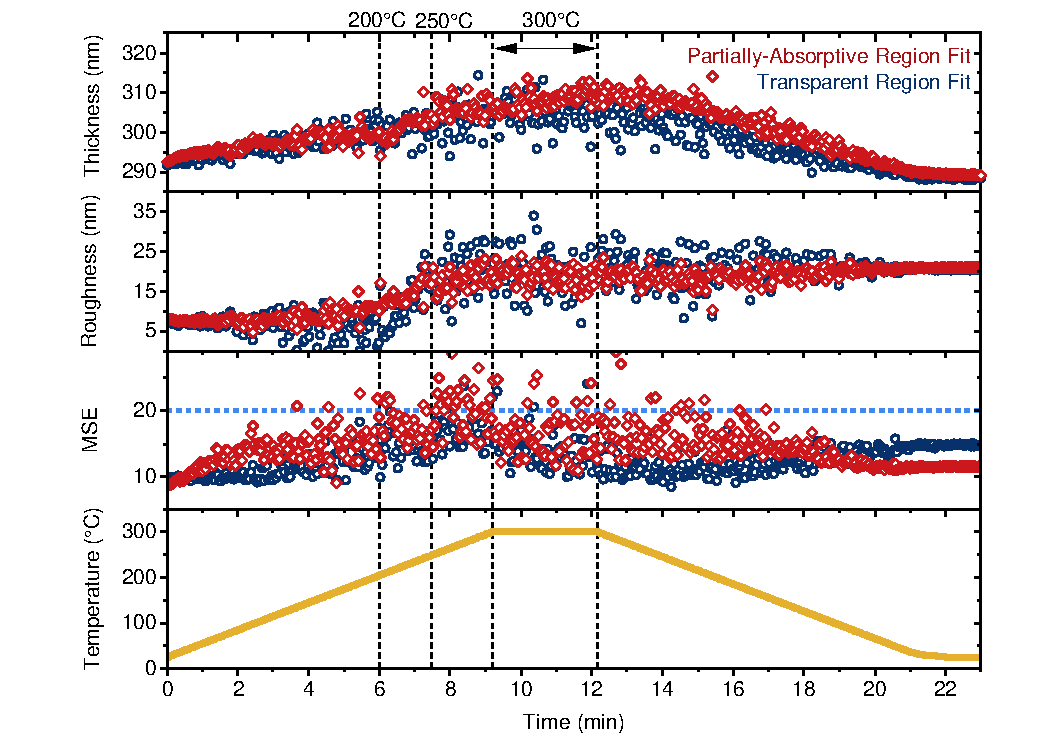
\includegraphics[width=.99\textwidth]{chapters/ellipsometry/image/Roughness_Thickness.pdf}
  \caption[Temperature effect on the perovskite's thickness and roughness according to the our dynamic SE model.]{Temperature effect on the perovskite's thickness and roughness according to the our dynamic SE model. For both parameters, there is a great agreement between the results of a Cauchy-based  (blue scatter points) in the transparent region (1000 - 2500 nm) and a Tauc-Lorentz-based model (red scatter points) in the partially absorptive region (300 - 1000 nm). For both models, the MSE is mostly maintained below 20 for the whole duration of the fit. A sharp increase in the film's roughness is triggered at 200\degree C, with the transition being completed at approximately 250 \degree C. Reproduced from \cite{Papadopoulou2024InEllipsometry}.}
  \label{fig:ellipsometry:roughness_thickness}
\end{figure}


As explained above, the changing properties of the perovskite thin film as a function of temperature can be described via an EMA model, which consists of 5 static models, mixed in different percentages. The dielectric functions of each static model are fixed, and only their volume ratio, along with the thickness of the bulk and roughness layers can vary. The percentage of voids in the roughness layer was again fixed at 15\%. Both the thickness and the optical constants of the \ch{SiO_2} layer are fixed, considering its particularly low thermal expansion coefficient ($0.5 \times 10^{-6} K^{-1}$), especially when compared to the thermal expansion coefficient of lead-iodide-based perovskites ($50\times10^{-6} K^{-1}$) \cite{Steele2019ThermalFilms}. Figure~\ref{fig:ellipsometry:roughness_thickness} shows the evolution of MSE as a function of time and temperature, which is mostly maintained below 20 for the whole duration of the experiment. This provides a preliminary indication of the accuracy of the dynamic model, which will be further corroborated in the following sections through comparisons with literature and the results from additional characterization measurements. 

\subsection{Impact of Annealing on Structural Properties}

Two types of scatter point are shown in Figure~\ref{fig:ellipsometry:roughness_thickness}. The red scatter points represent the fitting results of the dynamic model (Figure~\ref{fig:ellipsometry:dynamic_model}) in partially absorptive region (between 300 and 1000 nm). The blue scatter points represent the results of a simpler Cauchy-based model which is fitted in the transparent region (between 1000 and 2500 nm). The latter is not only more sensitive to thickness variations (due to light reflection from both the sample's surface and the sample-substrate interface),
but also simplifies the modeling of the roughness structure (the light wavelength is much larger compared to dimensions of the surface structure). As a result, the nearly identical trend in the evolution of the sample's thickness and roughness as a function of temperature that is observed between the two types of scatter points can further strengthen the confidence in the results of our dynamic model. 


\begin{figure}[htbp]
  \centering
  \medskip
  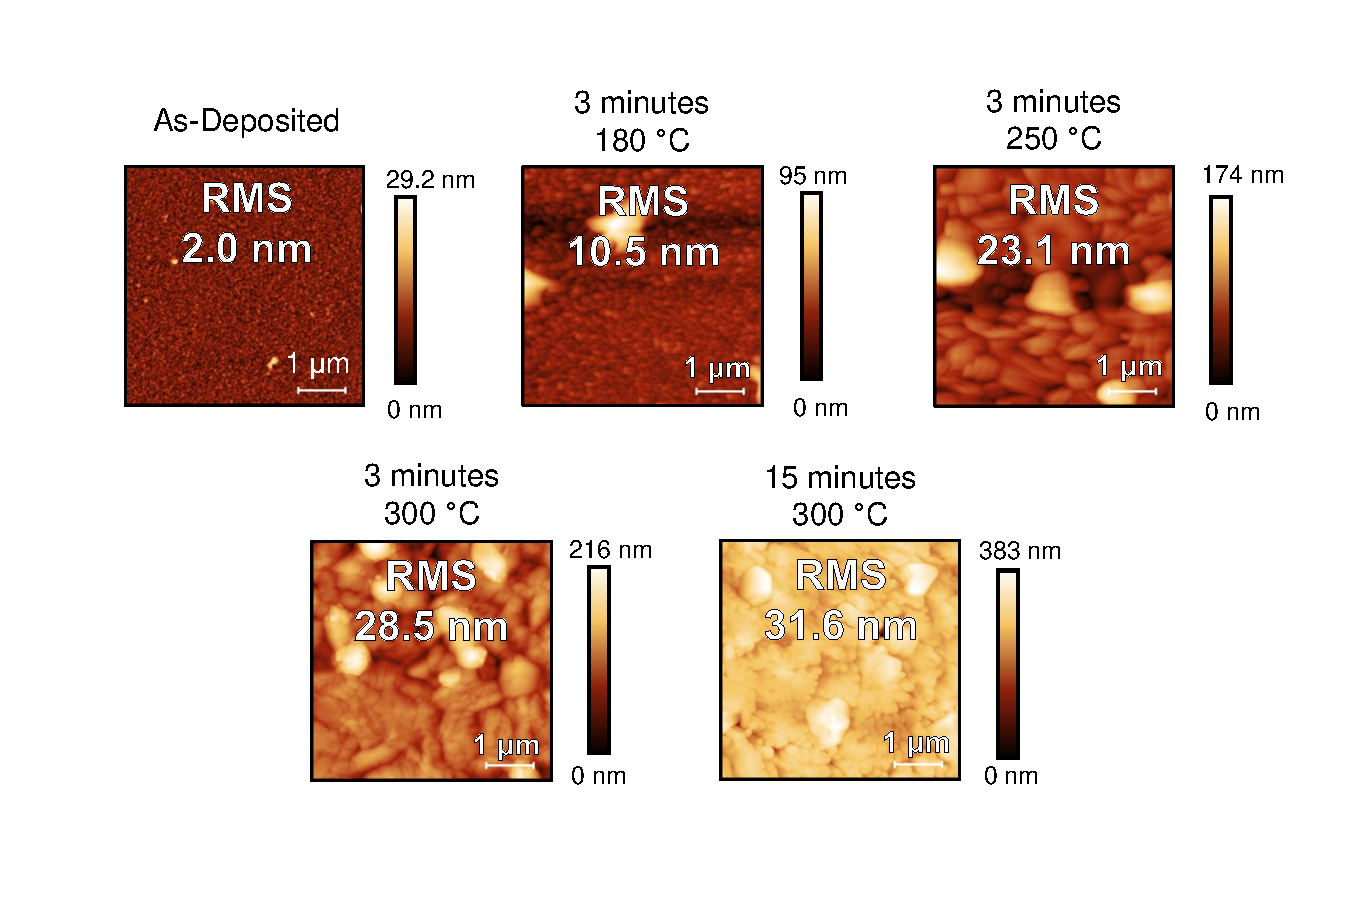
\includegraphics[width=1\textwidth]{chapters/ellipsometry/image/afm_all.pdf}
  \caption[AFM scans of \ch{CsPbI_2Br} thin films treated under various annealing conditions.]{AFM scans of \ch{CsPbI_2Br} thin films treated under various annealing conditions, including no annealing, 3 min at 180 \degree C, 3 min at 250 \degree C, 3 min at 300 \degree C, and 15 min at 300 \degree C. Adapted from \cite{Papadopoulou2024InEllipsometry}.}
  \label{fig:ellipsometry:afm_all}
\end{figure}


The results reveal that the sample's thickness is increasing linearly with temperature, despite the lattice phase changes that we know are happening. This is in agreement with what was observed by Marronnier et al, who used in situ synchrotron XRD measurements to report that the normalized unit cell volume of \ch{CsPbI_3} thin films varies linearly with temperature when transitioning sequentially from the the cubic to tetragonal and from tetragonal to orthorhombic phases \cite{Marronnier2018AnharmonicityCells}. Additionally, these results further agree with the high thermal expansion coefficient that has been reported for lead halide perovskites, with our films exhibiting a thickness increase in the range of $1.7\times10^{-4}K^{-1}$. Of course, this value is depends a lot on the type of substrate, and the substrate-induced stress, but should anyways be taken into account when designing perovskite-based components that are meant to be exposed to high processing or operating temperatures. 

The perovskites roughness shows an intriguing and potentially counter-intuitive behavior. It has been generally shown for solution-processed perovskite thin films that the longer the annealing duration the larger the size of grains eventually becomes \cite{Lee2019MicrostructuralCell}. Even though it is not possible to extract direct information about the size of the film's grains through an SE measurement, it has been previously shown that the simulated thickness of the model's roughness layer has a linear relationship with the film's real roughness, measured through AFM measurements \cite{Fujiwara2000AssessmentFilms}. Hence, it is logical to associate the SE-derived roughness value with the size of the film's grains. It is observed that the film's roughness remains mostly stable (between 5 and 10 nm) until approximately 200 \degree C. At this point, a sharp increase is observed, before the roughness stabilizes again to a value close to 20 nm. To validate these results, we submit different thermally evaporated \ch{CsPbI_2Br} films to various annealing conditions. Figure~\ref{fig:ellipsometry:afm_all} shows the AFM scan for a film annealed for 3 minutes at 180 \degree C and 250 \degree C, respectively. Indeed, when the temperature is maintained below 200 \degree C, the average grain size remains below 150 nm, similarly to the morphology of the as-deposited state, while when the annealing temperature exceeds 200 \degree C, the average grain size increases to a range between 400 and 800 nm. The temperature threshold for the grain coalescence seems to coincide with the transition from the tetragonal to the cubic phase (190 \degree C, as revealed through in situ GIWAXS). It remains unclear whether grain coalescence is a direct consequence of the phase transition or if both mechanisms merely share a similar activation energy. Regardless, the increase in surface roughness observed in the SE data could serve as a signature for evaluating the tetragonal-to-cubic phase transition temperature in alternative thermally evaporated perovskite compositions. Further increasing the annealing temperature (300 \degree C) or extending the annealing duration (300 \degree C for 15 minutes) results in only a minor increase in the film's RMS roughness (from 28.5 to 31.6 nm), consistent with the plateau in roughness observed it the SE results. This analysis highlights that the grain size of thermally evaporated perovskite thin films depends more on the nucleation during the growth of the crystal, rather than the post-deposition annealing step. Therefore, future efforts for improved film quality via larger grains should be focused on the crystallization mechanism during the deposition rather than post-deposition treatments. 


\subsection{Impact of Annealing on Optical Properties}

Beyond providing insights into the film's morphological evolution as a function of temperature, our proposed dynamic model also elucidates its impact on the film’s optical properties. This study not only enhances the fundamental understanding of crystal properties but also has direct applications across various fields. For example, the temperature dependence of a film's optical constants could serve as an input parameter for DFT simulations. Additionally, it can improve the prediction of the optoelectronic performance of perovskite-based devices operating at elevated temperatures, whether it is due to intrinsic factors (e.g., self-heating phenomena) or extrinsic factors (e.g., high ambient temperatures). Finally, this understanding could enable the design of photonic components with temperature-adjustable responses, allowing them to be fine-tuned for specific outputs (e.g. for optical phase shifting applications) \cite{Handa2019LargePerovskite}.

\begin{figure}
  \centering
  \medskip
  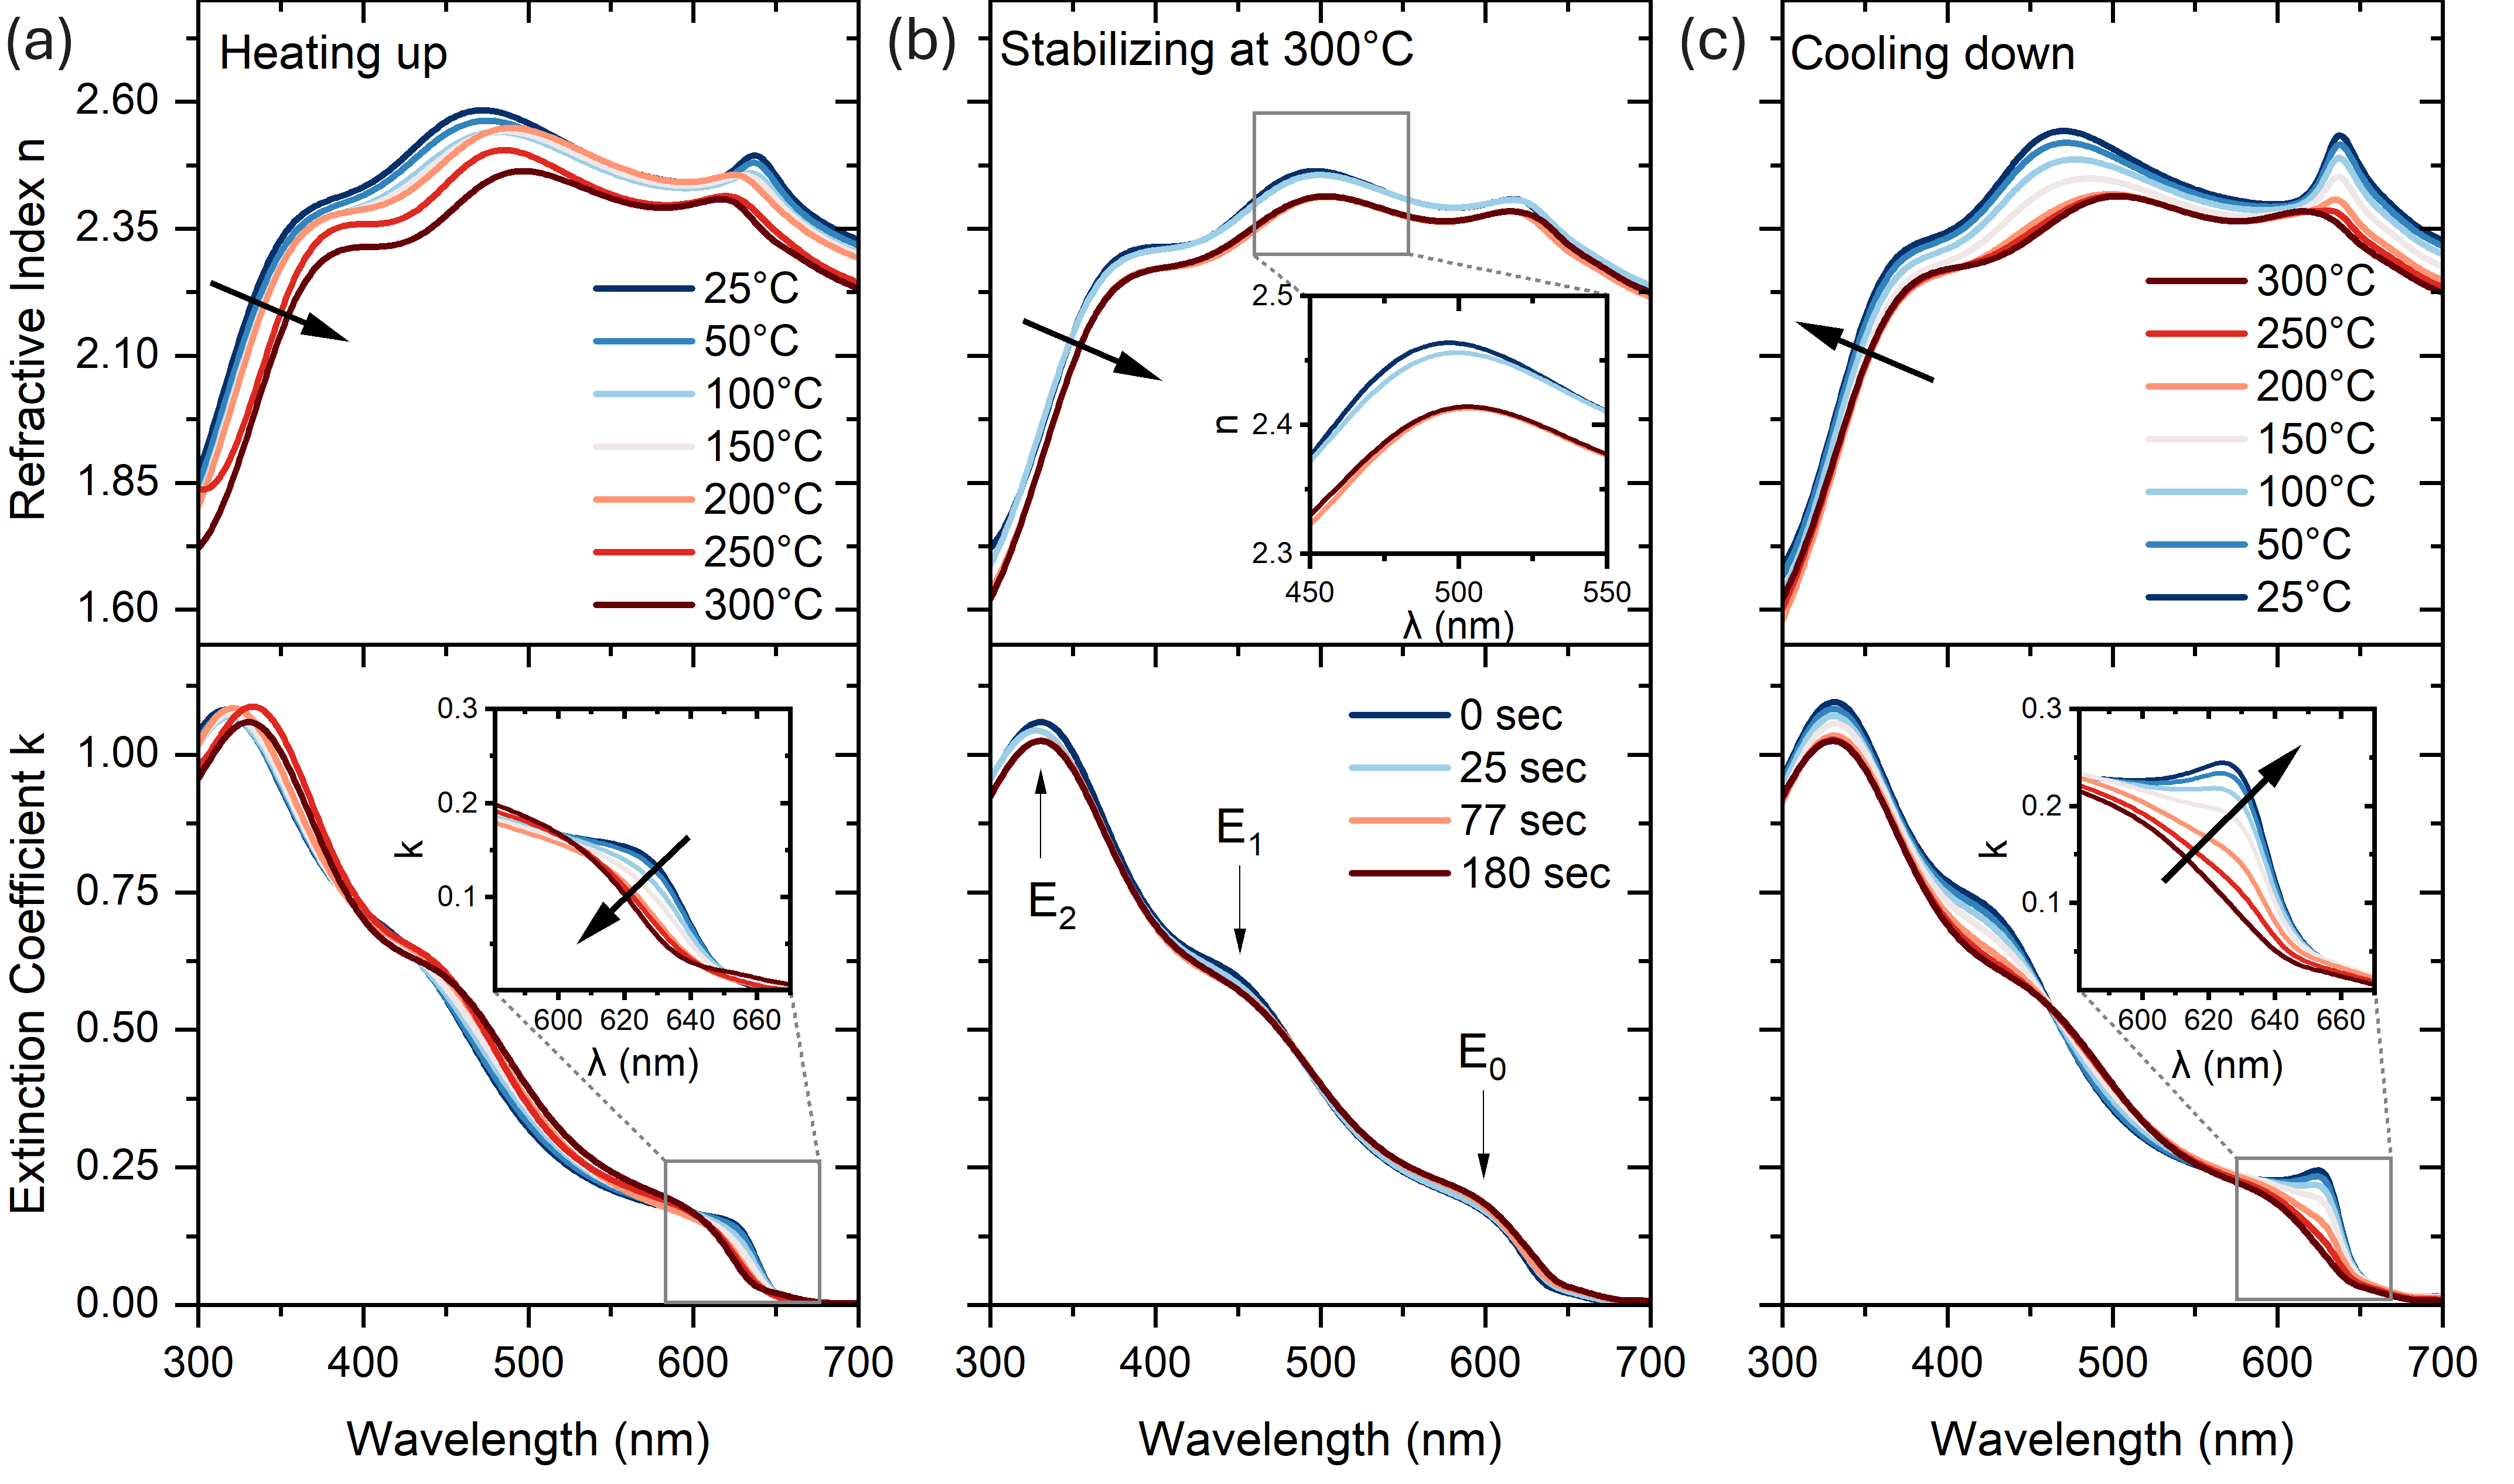
\includegraphics[width=.99\textwidth]{chapters/ellipsometry/image/Optical Constants_labeled.png}
  \caption[Temperature effect on the \ch{CsPbI_2Br} film's nk values during the heating, stabilizing at 300\degree C, and cooling down stages.]{Temperature effect on the \ch{CsPbI_2Br} film's nk values during the (a) heating, (b) stabilizing at 300\degree C, and (c) cooling down stages. With increasing temperature, the overall refractive index values decrease and the absorption edge in the film's extinction coefficient becomes less steep (and vice versa). These phenomena are attributed to the perovskite's negative thermo-optic coefficient and a rise in Urbach energy, respectively. Reproduced from \cite{Papadopoulou2024InEllipsometry}.}
  \label{fig:ellipsometry:optical_constants}
\end{figure}


Figure~\ref{fig:ellipsometry:optical_constants} provides a complete overview of the evolution of the film's optical constants during the various stages of the experiment, specifically during the heating up (Figure~\ref{fig:ellipsometry:optical_constants}a), the stabilizing at 300\degree C (Figure~\ref{fig:ellipsometry:optical_constants}b), and the cooling down (Figure~\ref{fig:ellipsometry:optical_constants}c) stages. It is evident that multiple changes occur simultaneously, highlighting the overall complexity of the temperature-dependent response of perovskite thin films. If we focus on the heating up stage of the experiment, the following changes can be observed: (i) a downwards shift of the refractive index, as well as (ii) a flattening of the absorption edge and (iii) an energy shift of the absorption peaks $E_0$, $E_1$, and $E_2$ in the extinction coefficient spectrum. The reverse trends can be observed during the cooling down stage, even though it is easy to notice some difference in the 25 \degree C spectrum before and after the annealing step, indicating the co-existence of reversible and non-reversible changes. The underlying physical mechanisms will be further detailed and explained in the following paragraphs. For the stage of stabilizing at 300\degree C, the spectrum of the extinction coefficient remains almost the same, even though an additional downwards shift can be observed in the refractive index. This characteristic is attributed to the relatively fast heating ramp ($\approx$ 30\degree C/min), and the subsequent delay between the attainment of a temperature point and the completion of potential transitions or internal structure changes. The results display that the film is reaching an equilibrium approximately 77 seconds after reaching  300 \degree C. It is important to highlight, that goal of this measurement is to observe the real-time evolution of thermally-evaporated \ch{CsPbI_2Br} thin films under the effect of increasing and decreasing temperature, rather than to precisely identify the temperature threshold for the occurrence of various mechanisms. 




\textbf{I. Thermo-Optic Coefficient Analysis}

It was previously mentioned that as the annealing temperature is increasing, the overall value of the refractive index across the whole spectrum is decreasing, and vice versa. The dependence of the refractive index on temperature is known as a material's thermo-optic coefficient ($dn/dT)$.  Most known and conventional semiconductor materials, such as Si, Ge, and GaN, are known to have a positive thermo-optic coefficient \cite{Fujiwara2018SpectroscopicCharacterization, Komma2012Thermo-opticTemperatures, Rao2022Temperature1550nm}. A positive thermo-optic coefficient  (i.e. increase of refractive index with increasing temperature) is a characteristic of low thermal expansion materials, where the light-matter interactions at higher temperatures are dominated by the reduction of the bandgap energy, and the consequent facilitation of electronic transitions. In contrast, hybrid organic-inorganic and quasi-2D perovskites were previously shown to possess a large negative thermo-optic coefficient \cite{Handa2019LargePerovskite, Wu2023CarrierPhononPerovskite}. Specifically, in the case of \ch{MAPbCl_3} single crystals, it was shown that $dn/dT = -3\times 10^{-4} K^{-1}$ at 430 nm \cite{Handa2019LargePerovskite}. The magnitude of this parameter was attributed to the large expansion coefficient of perovskite thin films, and the consequent decrease in the valence electron density with increasing temperature, which in turn limits the interaction of light with the material \cite{Handa2020LargeCH4NH3PbCl3}. 


\begin{figure}[htbp]
    \centering
    \begin{subfigure}{0.32\textwidth}
        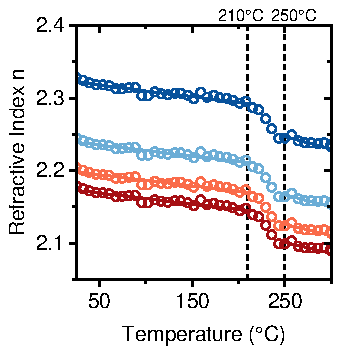
\includegraphics[width=\textwidth]{chapters/ellipsometry/image/Thermo-optic_Coefficient_heating.pdf}
        \caption{}
        \label{fig:ellipsometry:thermooptic_heating}
    \end{subfigure}
    \hfill
    \begin{subfigure}{0.32\textwidth}
        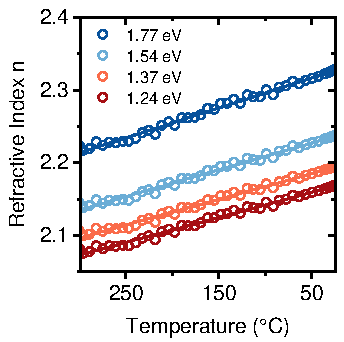
\includegraphics[width=\textwidth]{chapters/ellipsometry/image/Thermo-optic_Coefficient_cooling.pdf}
        \caption{}
        \label{fig:ellipsometry:thermooptic_cooling}
    \end{subfigure}
    \hfill
    \begin{subfigure}{0.3\textwidth}
        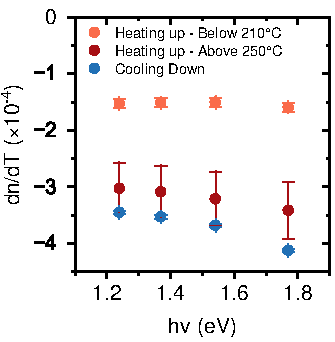
\includegraphics[width=\textwidth]{chapters/ellipsometry/image/Thermo-optic_Coefficient_energy.pdf}
        \caption{}
        \label{fig:ellipsometry:thermooptic_energy}
    \end{subfigure}
    \caption[Impact of temperature on the perovskite's refractive index for photons with the sub-bandgap energies during the heating and cooling down stages.]{Impact of temperature on the perovskite's refractive index for photons with the sub-bandgap energies during the (a) heating and (b) cooling down stages. A linear fit is performed to extract the film's (c) thermo-optic coefficient (dn/dT). Reproduced from \cite{Papadopoulou2024InEllipsometry}.}
    \label{fig:ellipsometry:thermooptic}
\end{figure}

Considering that the thermo-optic coefficient depends on the energy of incident light, Figure~\ref{fig:ellipsometry:thermooptic_heating} and Figure~\ref{fig:ellipsometry:thermooptic_cooling} present the variation of the film's refractive index as a function of temperature for four sub-bandgap energies, during the heating and cooling stages, respectively. For the former, n shows a linear dependence on temperature up to 200 \degree C, where a sharp discontinuity is observed. The relevant transition is completed when the temperature reaches 250 \degree C. During the cooling stage, n maintains a linear relationship to temperature for the complete duration of the cooling ramp. The thermo-optic coefficient is extracted through a linear fit on each region of interest, with results being presented in Figure~\ref{fig:ellipsometry:thermooptic_energy}. The extracted values vary in the range of -1.5 and $-4.5\times 10^{-4} K^{-1}$, which is close to the value previously reported for \ch{MAPbCl_3} single crystals. The sharp discontinuity of the thermo-optic coefficient during the heating stage coincides with increase in the roughness profile of the film, as was already shown in Figure~\ref{fig:ellipsometry:roughness_thickness}. It should be noted that an increase in film roughness in an SE model is represented as a thickness increase of an EMA layer, which consists of a mixture of the bulk material and voids. Therefore, the correlation between the film's roughness and thermo-optic coefficient could be justified considering the dependence of the latter on the expansion of the film.


\textbf{II. Urbach Tail Analysis}

The next part of this analysis focuses on the dependence of the slope of the extinction coefficient's absorption edge on temperature. The insets of Figure~\ref{fig:ellipsometry:optical_constants}a and Figure~\ref{fig:ellipsometry:optical_constants}c, clearly demonstrate that slope of the absorption edge is becoming less steep with increasing temperature, and vice versa. To further understand and explain this phenomenon it is important to introduce the parameter of Urbach energy ($E_U$), which quantifies the slope of the absorption edge, describing the energetic disorder of the material \cite{Urbach1953TheSolids,Rajagopal2017DefectPhotovoltaics}. This can be better understood by considering that the slope of the absorption edge is strongly influenced by sub-bandgap absorption tails, with more pristine materials exhibiting steeper absorption edges \cite{Zhang2022UnravelingDisorder}. As a result, small $E_U$ values are typically associated with superior optoelectronic properties, including lower carrier recombination and higher mobilities \cite{Zhang2022UnravelingDisorder, Ledinsky2019TemperaturePerovskites}. The Urbach energy can be quantified through the empirical relation: 

\begin{equation}
    a(hv) = a_0exp(\frac{hv}{E_U}),
    \label{eq:urbach_absorption}
\end{equation}

where $a$ is the material's absorption coefficient, $a_0$ is a constant, and $hv$ is the incident photon energy. The dependence of $E_U$ on temperature is further described by the equation \cite{Kurik1971UrbachRule}: 

\begin{equation}
    E_U(T) = E_U(0) + \frac{2E_U(0)}{e^{\theta_E /T}-1}.
    \label{eq:urbach_temp}
\end{equation}

Eq.~\ref{eq:urbach_temp} can be distinguished into two components, a static one ($E_U(0)$), which is temperature independent, describing the intrinsic disorder of the material, and a dynamic one, which describes the phonon contribution. In the dynamic term of the equation, T is the absolute temperature and $\theta_E$ is the Einstein phonon temperature. It has to be noted that static disorder dominates at temperatures below 150 K, so the results presented here are mostly influenced by dynamic disorder and exciton-phonon interactions \cite{Zhang2022UnravelingDisorder}.


\begin{figure}[htbp]
    \centering
    \begin{subfigure}{0.32\textwidth}
        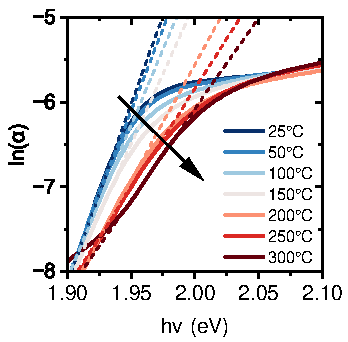
\includegraphics[width=\textwidth]{chapters/ellipsometry/image/Urbach_heating.pdf}
        \caption{}
        \label{fig:ellipsometry:urbach_heating}
    \end{subfigure}
    \hfill
    \begin{subfigure}{0.32\textwidth}
        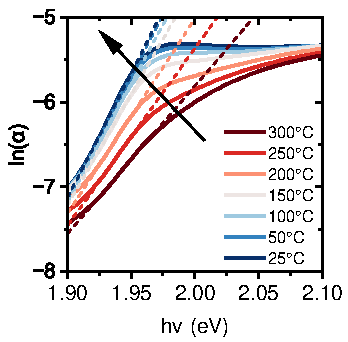
\includegraphics[width=\textwidth]{chapters/ellipsometry/image/Urbach_cooling.pdf}
        \caption{}
        \label{fig:ellipsometry:urbach_cooling}
    \end{subfigure}
    \hfill
    \begin{subfigure}{0.3\textwidth}
        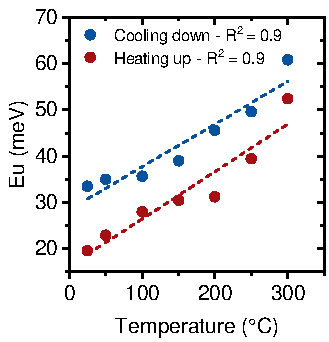
\includegraphics[width=\textwidth]{chapters/ellipsometry/image/Urbach_temp.pdf}
        \caption{}
        \label{fig:ellipsometry:urbach_temp}
    \end{subfigure}
    \caption[Impact of temperature on the perovskite's absorption edge during the heating and cooling down stages.]{Impact of temperature on the perovskite's absorption edge, expressed through the natural logarithm of the absorption coefficient, during the (a) heating and (b) cooling down stages. (c) Urbach energy as a function of temperature, as extracted through eq.~\ref{eq:urbach_absorption}. Reproduced from \cite{Papadopoulou2024InEllipsometry}.}
    \label{fig:ellipsometry:urbach}
\end{figure}

In terms of perovskite research, the Urbach energy has been quantified for thin films and single crystals utilizing measurements such as photothermal deflection spectroscopy, Fourier transform photocurrent spectroscopy, and time-integrated and time-resolved photoluminescence measurements \cite{Zhang2022UnravelingDisorder, Ledinsky2019TemperaturePerovskites, Singh2016EffectCH3NH3PbI3, DeWolf2014OrganometallicPerformance, Falsini2022AnalysisPerovskites}. These studies have primarily focused on temperatures from RT and below. However, the study of the Urbach Energy of thermally evaporated perovskite thin films has not yet been investigated, while the extension of the temperature range above RT is highly relevant considering the correlation between $E_U$ and critical device parameters, such as the $V_{oc}$ of solar cells, and consequently the dark current of photodiodes \cite{Ledinsky2019TemperaturePerovskites}.

In order to extract $E_U$ according to Eq.~\ref{eq:urbach_absorption}, it is necessary to calculate the film's absorption coefficient using the extinction coefficient spectrum ($a = \frac{4\pi k}{\lambda}$). Figure~\ref{fig:ellipsometry:urbach_heating} and Figure~\ref{fig:ellipsometry:urbach_cooling} present the natural logarithm of the absorption coefficient as a function of photon energy for various temperature intervals during the heating and cooling stages, respectively. $E_U$ can be following quantified through the slope of the linear fit, with Figure~\ref{fig:ellipsometry:urbach_temp} showing $E_U$ as a function of temperature for the heating and cooling stages. 

A linear dependence of $E_U$ on temperature can be observed for both stages. In a prior study on the temperature dependence of $E_U$ for \ch{CH_3NH_3PbI_3} films by Singh et al., it was shown that the orthorhombic-to-tetragonal phase transition can be identified through a minor slope change \cite{Singh2016EffectCH3NH3PbI3}. However, the use of a relatively fast and continuous heating ramp in our case, without stabilization intervals, leads to a more gradual transition and potential co-existence of phases. Therefore, it is not possible to identify specific structural transitions. Additionally, the $E_U$ values of the cooling stage display an upwards shift compared to the respective values of the heating stage. For reference, $E_U$ at RT for the as-deposited sate is approximately equal to 19 meV, which indicates a well-ordered microstructure. The same value for the annealed state at RT is approximately equal to 33 meV, displaying a 14 meV increase. Considering that both measurements were carried out at the same temperature, Eq.~\ref{eq:urbach_temp} indicates that the $E_U$ increase can only be attributed to the static term of the equation, i.e. an increase in the structural disorder. This finding comes in contrast to what was discussed in Sec.~\ref{sec:ex_situ}, which highlighted the improvements in crystalline quality of the film after the annealing step. As a result, the increase in $E_U$ is rather attributed to the temperature-induced strain in the lattice, which was already indicated as a peak splitting in the GIWAXS data presented in Figure~\ref{fig:ch2:giwaxs_before_after:} \cite{Kim2020ImpactCells}. 



\textbf{III. Critical Point Analysis}


The last part of this section is dedicated to the interpretation of the energy shifts of the absorption peaks (labeled as $E_0$, $E_1$, and $E_2$ in Figure~\ref{fig:ellipsometry:optical_constants}) as a function of temperature. These peaks, known as critical points (CPs), are a fundamental characteristic of a material's dielectric function and are associated with interband transitions at high-symmetry k-points of the Brillouin zone \cite{Aspnes1983DielectricEV}. Even though these features are already prominent in the refractive index and extinction coefficient, a systematic analysis relies on the attainment of the second derivative of the dielectric function spectra, which not only enhances structural features, but suppresses spectral noise, as well. Each CP is described by the equation: 

\begin{equation}
    \frac{\partial ^2\epsilon}{\partial \omega^2} = n(n-1)Ae^{i\Phi}(\omega -E +i\Gamma)^{(n-2)},
    \label{eq:critical_point}
\end{equation}

where $A$, $\Phi$, $E$, and $\Gamma$ describe the amplitude, phase, energy position, and broadening of the CP. The dimensionality of the CP, is defined by $n$, which is set equal to -1/2, 0, +1/2 for 1-D, 2-D, and 3-D transitions, respectively. Excitonic transitions, which were previously used to describe optical transition in perovskites, are represented by $n=-1$ \cite{Jiang2016TemperatureEllipsometry, Ceratti2021CsPbBr3Air}. These parameters can be obtained through a regression analysis of the experimental derivative with the theoretical lineshapes of Eq.~\ref{eq:critical_point}. Figure~\ref{fig:ellipsometry:deriv} illustrates the fitting results on the real ($\epsilon_r$) and imaginary ($\epsilon_i$) part of the dielectric function for different stages of our experiment, considering the presence of three CPs, indicating a good match between experimental and simulated values. 

\begin{figure}[ht!]
    \centering
    \begin{subfigure}{0.34\textwidth}
        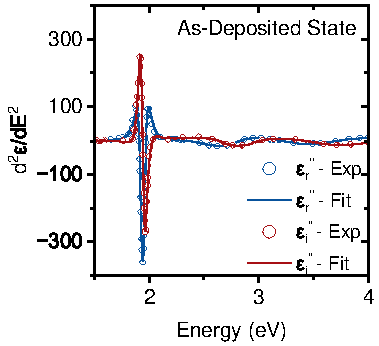
\includegraphics[width=\textwidth]{chapters/ellipsometry/image/Deriv_As_Dep.pdf}
        \caption{}
        \label{fig:ellipsometry:deriv:As_dep}
    \end{subfigure}
    \hfill
    \begin{subfigure}{0.31\textwidth}
        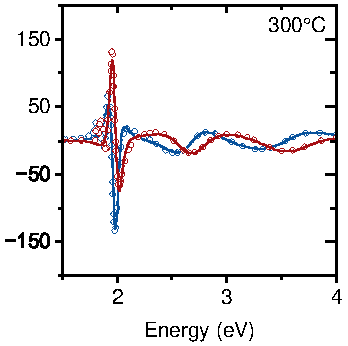
\includegraphics[width=\textwidth]{chapters/ellipsometry/image/Deriv_300C.pdf}
        \caption{}
        \label{fig:ellipsometry:deriv:300}
    \end{subfigure}
    \hfill
    \begin{subfigure}{0.31\textwidth}
        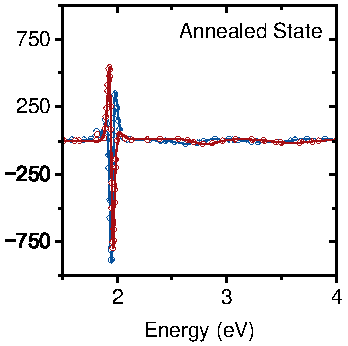
\includegraphics[width=\textwidth]{chapters/ellipsometry/image/Deriv_Anneal.pdf}
        \caption{}
        \label{fig:ellipsometry:deriv:anneal}
    \end{subfigure}
    \caption[Second-order derivatives of the real and imaginary part of the film's dielectric function for the as-deposited state, the state at 300\degree C, and the annealed state.]{Second-order derivatives of the real and imaginary part of the film's dielectric function for the (a) as-deposited state, (b) the state at 300\degree C, and (c) the annealed state. The solid line represents the fit of eq.~\ref{eq:critical_point} on the experimental data. The density of scatter points has been reduced for a more clear visualization. Reproduced from \cite{Papadopoulou2024InEllipsometry}.}
    \label{fig:ellipsometry:deriv}
\end{figure}


The most pronounced feature in Figure~\ref{fig:ellipsometry:deriv}a-c represents the fundamental direct bandgap of the perovskite thin film ($E_0$), which is defined by the antibonding of Pb and halogen orbitals \cite{Mannino2020Temperature-DependentCrystals}. For an $\alpha$-\ch{CsPbI_2Br} thins films, $E_0$ results from the interband transition at the R point in the first Brillouin zone. The two additional, but less pronounced, CPs ($E_1$ and $E_2$) are mainly caused by the interband transitions at the M and X point of the Brillouin zone, respectively. From a physical point of view, $E_1$ is attributed to transitions from the 6s and 6p orbits in the \ch{Pb^{2+}} sublattice, while $E_2$ is a doublet transition owing to the charge-transfer transitions form the I/Br 3p/4p valence to the Pb 6p conduction bands \cite{Zhao2018EllipsometricFilm}.   


\begin{figure}[ht!]
    \centering
    \begin{subfigure}{0.34\textwidth}
        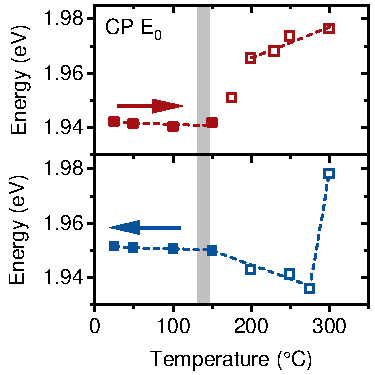
\includegraphics[width=\textwidth]{chapters/ellipsometry/image/CP0.pdf}
        \caption{}
        \label{fig:ellipsometry:CP0}
    \end{subfigure}
    \hfill
    \begin{subfigure}{0.31\textwidth}
        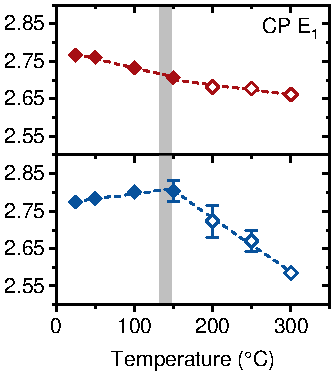
\includegraphics[width=\textwidth]{chapters/ellipsometry/image/CP1.pdf}
        \caption{}
        \label{fig:ellipsometry:CP1}
    \end{subfigure}
    \hfill
    \begin{subfigure}{0.31\textwidth}
        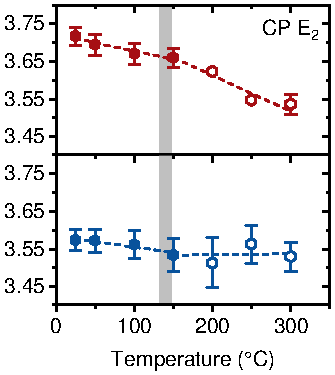
\includegraphics[width=\textwidth]{chapters/ellipsometry/image/CP3}
        \caption{}
        \label{fig:ellipsometry:deriv:CP2}
    \end{subfigure}
    \caption[Impact of temperature on the energy position of interband critical points during the heating and cooling stages.]{Impact of temperature on the energy position of interband critical points (a) $E_0$, (b) $E_1$, and (c) $E_2$ during the heating (red scatter points) and the cooling (blue scatter points) stages. The temperature point for the transition between the orthorhombic (filled scatter points) and the tetragonal (empty scatter points) phases is indicated by the shaded area. Reproduced from \cite{Papadopoulou2024InEllipsometry}.}
    \label{fig:ellipsometry:CP_all}
\end{figure}


Figure~\ref{fig:ellipsometry:CP_all}a-c illustrate the energy position of the three CPs as a function of temperature for the heating and cooling stage of the experiment. The extracted values of the fundamental bandgap at RT (1.94 - 1.95 eV) are in good agreement with what has been previously reported for the \ch{CsPbI_2Br} composition \cite{Yuan2021Moisture-stimulatedProperties, Chen2019ThePerovskite,Parida2019Two-stepStability, Igual-Munoz2020Room-TemperaturePrecursors, Mali2021ImplementingCells}. During the heating ramp, $E_0$ is displaying blueshift, while $E_1$ and $E_2$ display a redshift, which is in agreement with what was previously reported for \ch{CsPbBr_3} single crystals \cite{Ceratti2021CsPbBr3Air}. The blueshift of $E_0$ can be further understood considering the dependence of the later on the lattice's expansion and consequent increase in interatom distance, which in turn leads to a lowering of the valence band minimum. Additionally, a sharp discontinuity is observed for all CPs at 140 \degree C, which according the GIWAXS data presented earlier (Figure~\ref{fig:ch2:giwaxs_insitu}) coincides with the transition between the orthorhombic and tetragonal phases. The same discontinuity was also observed for \ch{CsPbBr_3} single crystals \cite{Mannino2020Temperature-DependentCrystals}. It is known that $E_0$ has a dependence on the tilting of the [\ch{PbX_6^{4-}}] octahedra, which is directly responsible for the aforementioned phase transition, potentially explaining the origin of the discontinuity. As a result, this feature in the results of the dynamic SE model could be used as a fingerprint for the identification of the tetragonal-to-orthorhombic phase transition for the characterization of additional compositions, as an alternative to using synchrotron-based techniques, such as GIWAXS. On the other hand, the tetragonal-to-cubic phase transition (at approximately 200 \degree C) does not exhibit any distinguishable features, potentially attributed to the continuous tilting of the \ch{PbX_6} octahedra and the continuous change of the Pb-X bond lengths as a function of temperature \cite{Foley2015TemperaturePerovskite}. An exception to the observed trends is the energy variation of CP $E_0$ during cooling, which shows a sharp drop at the onset of the cooling process. Further investigation is required to understand this behavior.



\section{Conclusions}

In conclusion, this chapter has provided a comprehensive evaluation of the impact of thermal annealing on co-evaporated \ch{CsPbI_2Br} thin films. It was found that the as-deposited films already exhibit the black perovskite phase, attributed to the in situ reaction of the precursors on the substrate. However, the initial grain size is relatively small (below 50 nm), which increases significantly to a range of 100–800 nm after a post-deposition annealing step. This thermal treatment also leads to a threefold increase in SSPL intensity and doubles the carrier lifetime. GIWAXS analysis reveals that, following annealing, the film reverts to the $\gamma$-phase, accompanied by the emergence of a 0D \ch{Cs_4PbI_4Br_2} phase—likely a consequence of excess CsBr introduced during the co-evaporation process.

The second part of this chapter explores the use of spectroscopic ellipsometry from a novel perspective, focusing on its application in monitoring real-time annealing effects on thermally evaporated thin films. Specifically, we introduce a computationally efficient dynamic model capable of capturing the evolution of the film’s structural and optical properties during annealing. Particular attention is given to the modeling of films with increasing surface roughness, which is effectively represented by adjusting the void fraction in the model's roughness layer. Careful analysis reveals that the $\gamma$-to-$\beta$ phase transition manifests as a discontinuity in the energy position of the fundamental bandgap, while the $\beta$-to-$\alpha$ transition is marked by a pronounced increase in surface roughness. Additionally, this study discusses the temperature dependence of key parameters such as the film’s thermo-optic coefficient and Urbach energy, offering further insight into the thermally induced changes. 

Looking ahead, the dynamic modeling approach presented for analyzing temperature-dependent SE spectra holds significant potential for future investigations. One example could involve exploring the impact of the substrate, including different transport layers, on the growth and crystallization of thermally evaporated perovskite thin films. In such cases, an initial temperature-dependent SE study on the selected transport layers is essential to determine whether their optical and structural properties can be regarded as temperature-independent. For transport layers that exhibit temperature sensitivity (such as organic materials with high thermal expansion coefficients) dedicated dynamic models should be developed to describe their behavior, following a similar approach to the one presented in this chapter.

%%%%%%%%%%%%%%%%%%%%%%%%%%%%%%%%%%%%%%%%%%%%%%%%%%
% Keep the following \cleardoublepage at the end of this file, 
% otherwise \includeonly includes empty pages.
\cleardoublepage

